\documentclass[twoside]{book}

% Packages required by doxygen
\usepackage{fixltx2e}
\usepackage{calc}
\usepackage{doxygen}
\usepackage[export]{adjustbox} % also loads graphicx
\usepackage{graphicx}
\usepackage[utf8]{inputenc}
\usepackage{makeidx}
\usepackage{multicol}
\usepackage{multirow}
\PassOptionsToPackage{warn}{textcomp}
\usepackage{textcomp}
\usepackage[nointegrals]{wasysym}
\usepackage[table]{xcolor}

% NLS support packages
\usepackage[spanish]{babel}
% Font selection
\usepackage[T1]{fontenc}
\usepackage[scaled=.90]{helvet}
\usepackage{courier}
\usepackage{amssymb}
\usepackage{sectsty}
\renewcommand{\familydefault}{\sfdefault}
\allsectionsfont{%
  \fontseries{bc}\selectfont%
  \color{darkgray}%
}
\renewcommand{\DoxyLabelFont}{%
  \fontseries{bc}\selectfont%
  \color{darkgray}%
}
\newcommand{\+}{\discretionary{\mbox{\scriptsize$\hookleftarrow$}}{}{}}

% Page & text layout
\usepackage{geometry}
\geometry{%
  a4paper,%
  top=2.5cm,%
  bottom=2.5cm,%
  left=2.5cm,%
  right=2.5cm%
}
\tolerance=750
\hfuzz=15pt
\hbadness=750
\setlength{\emergencystretch}{15pt}
\setlength{\parindent}{0cm}
\setlength{\parskip}{3ex plus 2ex minus 2ex}
\makeatletter
\renewcommand{\paragraph}{%
  \@startsection{paragraph}{4}{0ex}{-1.0ex}{1.0ex}{%
    \normalfont\normalsize\bfseries\SS@parafont%
  }%
}
\renewcommand{\subparagraph}{%
  \@startsection{subparagraph}{5}{0ex}{-1.0ex}{1.0ex}{%
    \normalfont\normalsize\bfseries\SS@subparafont%
  }%
}
\makeatother

% Headers & footers
\usepackage{fancyhdr}
\pagestyle{fancyplain}
\fancyhead[LE]{\fancyplain{}{\bfseries\thepage}}
\fancyhead[CE]{\fancyplain{}{}}
\fancyhead[RE]{\fancyplain{}{\bfseries\leftmark}}
\fancyhead[LO]{\fancyplain{}{\bfseries\rightmark}}
\fancyhead[CO]{\fancyplain{}{}}
\fancyhead[RO]{\fancyplain{}{\bfseries\thepage}}
\fancyfoot[LE]{\fancyplain{}{}}
\fancyfoot[CE]{\fancyplain{}{}}
\fancyfoot[RE]{\fancyplain{}{\bfseries\scriptsize Generado por Doxygen }}
\fancyfoot[LO]{\fancyplain{}{\bfseries\scriptsize Generado por Doxygen }}
\fancyfoot[CO]{\fancyplain{}{}}
\fancyfoot[RO]{\fancyplain{}{}}
\renewcommand{\footrulewidth}{0.4pt}
\renewcommand{\chaptermark}[1]{%
  \markboth{#1}{}%
}
\renewcommand{\sectionmark}[1]{%
  \markright{\thesection\ #1}%
}

% Indices & bibliography
\usepackage{natbib}
\usepackage[titles]{tocloft}
\setcounter{tocdepth}{3}
\setcounter{secnumdepth}{5}
\makeindex

% Hyperlinks (required, but should be loaded last)
\usepackage{ifpdf}
\ifpdf
  \usepackage[pdftex,pagebackref=true]{hyperref}
\else
  \usepackage[ps2pdf,pagebackref=true]{hyperref}
\fi
\hypersetup{%
  colorlinks=true,%
  linkcolor=blue,%
  citecolor=blue,%
  unicode%
}

% Custom commands
\newcommand{\clearemptydoublepage}{%
  \newpage{\pagestyle{empty}\cleardoublepage}%
}

\usepackage{caption}
\captionsetup{labelsep=space,justification=centering,font={bf},singlelinecheck=off,skip=4pt,position=top}

%===== C O N T E N T S =====

\begin{document}

% Titlepage & ToC
\hypersetup{pageanchor=false,
             bookmarksnumbered=true,
             pdfencoding=unicode
            }
\pagenumbering{alph}
\begin{titlepage}
\vspace*{7cm}
\begin{center}%
{\Large Proyecto S\+O\+P\+ER }\\
\vspace*{1cm}
{\large Generado por Doxygen 1.8.13}\\
\end{center}
\end{titlepage}
\clearemptydoublepage
\pagenumbering{roman}
\tableofcontents
\clearemptydoublepage
\pagenumbering{arabic}
\hypersetup{pageanchor=true}

%--- Begin generated contents ---
\chapter{Índice de clases}
\section{Lista de clases}
Lista de las clases, estructuras, uniones e interfaces con una breve descripción\+:\begin{DoxyCompactList}
\item\contentsline{section}{\hyperlink{structMensaje}{Mensaje} }{\pageref{structMensaje}}{}
\item\contentsline{section}{\hyperlink{structtipo__casilla}{tipo\+\_\+casilla} }{\pageref{structtipo__casilla}}{}
\item\contentsline{section}{\hyperlink{structtipo__mapa}{tipo\+\_\+mapa} }{\pageref{structtipo__mapa}}{}
\item\contentsline{section}{\hyperlink{structtipo__nave}{tipo\+\_\+nave} }{\pageref{structtipo__nave}}{}
\end{DoxyCompactList}

\chapter{Indice de archivos}
\section{Lista de archivos}
Lista de todos los archivos documentados y con descripciones breves\+:\begin{DoxyCompactList}
\item\contentsline{section}{src/\hyperlink{gamescreen_8c}{gamescreen.\+c} \\*Código fuente del modo pantalla }{\pageref{gamescreen_8c}}{}
\item\contentsline{section}{src/\hyperlink{gamescreen_8h}{gamescreen.\+h} \\*Cabecera del modo pantalla }{\pageref{gamescreen_8h}}{}
\item\contentsline{section}{src/\hyperlink{jefe_8c}{jefe.\+c} \\*Código fuente de jefe }{\pageref{jefe_8c}}{}
\item\contentsline{section}{src/\hyperlink{jefe_8h}{jefe.\+h} \\*Recoge la funcionalidad de un jefe }{\pageref{jefe_8h}}{}
\item\contentsline{section}{src/\hyperlink{mapa_8c}{mapa.\+c} \\*Código fuente del mapa }{\pageref{mapa_8c}}{}
\item\contentsline{section}{src/\hyperlink{mapa_8h}{mapa.\+h} \\*Cabecera del mapa }{\pageref{mapa_8h}}{}
\item\contentsline{section}{src/\hyperlink{monitor_8c}{monitor.\+c} \\*Código fuente del monitor }{\pageref{monitor_8c}}{}
\item\contentsline{section}{src/\hyperlink{nave_8c}{nave.\+c} \\*Codigo fuente de nave }{\pageref{nave_8c}}{}
\item\contentsline{section}{src/\hyperlink{nave_8h}{nave.\+h} \\*Recoge la funcionalidad de una nave }{\pageref{nave_8h}}{}
\item\contentsline{section}{src/\hyperlink{simulador_8c}{simulador.\+c} \\*Código fuente del simulador }{\pageref{simulador_8c}}{}
\item\contentsline{section}{src/\hyperlink{types_8h}{types.\+h} \\*Define los tipos y constantes de datos }{\pageref{types_8h}}{}
\end{DoxyCompactList}

\chapter{Documentación de las clases}
\hypertarget{structMensaje}{}\section{Referencia de la Estructura Mensaje}
\label{structMensaje}\index{Mensaje@{Mensaje}}
\subsection*{Atributos públicos}
\begin{DoxyCompactItemize}
\item 
\mbox{\Hypertarget{structMensaje_a4e71da8fc67abc10c724df97194b7634}\label{structMensaje_a4e71da8fc67abc10c724df97194b7634}} 
char {\bfseries info} \mbox{[}\hyperlink{types_8h_ae0b4816fb45161ef9da5e6d6134ee28a}{T\+AM}\mbox{]}
\item 
\mbox{\Hypertarget{structMensaje_aca66756f8b0eabb4d54e5ad57658c6d4}\label{structMensaje_aca66756f8b0eabb4d54e5ad57658c6d4}} 
int {\bfseries n\+\_\+nave}
\item 
\mbox{\Hypertarget{structMensaje_ae67ecce3997185e65960fb5b32334258}\label{structMensaje_ae67ecce3997185e65960fb5b32334258}} 
int {\bfseries n\+\_\+equipo}
\item 
\mbox{\Hypertarget{structMensaje_ac3b6a217eefdd69948b675c9410045c2}\label{structMensaje_ac3b6a217eefdd69948b675c9410045c2}} 
int {\bfseries x}
\item 
\mbox{\Hypertarget{structMensaje_a4503e89a9f6a07a0a99fb4bed4cc8e6f}\label{structMensaje_a4503e89a9f6a07a0a99fb4bed4cc8e6f}} 
int {\bfseries y}
\end{DoxyCompactItemize}


La documentación para esta estructura fue generada a partir del siguiente fichero\+:\begin{DoxyCompactItemize}
\item 
src/\hyperlink{types_8h}{types.\+h}\end{DoxyCompactItemize}

\hypertarget{structtipo__casilla}{}\section{Referencia de la Estructura tipo\+\_\+casilla}
\label{structtipo__casilla}\index{tipo\+\_\+casilla@{tipo\+\_\+casilla}}
\subsection*{Atributos públicos}
\begin{DoxyCompactItemize}
\item 
\mbox{\Hypertarget{structtipo__casilla_a028b6f19741cf3492c595a2868175fd5}\label{structtipo__casilla_a028b6f19741cf3492c595a2868175fd5}} 
char \hyperlink{structtipo__casilla_a028b6f19741cf3492c595a2868175fd5}{simbolo}
\begin{DoxyCompactList}\small\item\em Símbolo que se mostrará en la pantalla para esta casilla. \end{DoxyCompactList}\item 
\mbox{\Hypertarget{structtipo__casilla_aa0d456b8dc9a45dc12fd1018f971823f}\label{structtipo__casilla_aa0d456b8dc9a45dc12fd1018f971823f}} 
int \hyperlink{structtipo__casilla_aa0d456b8dc9a45dc12fd1018f971823f}{equipo}
\begin{DoxyCompactList}\small\item\em Si está vacia = -\/1. Si no, número de equipo de la nave que está en la casilla. \end{DoxyCompactList}\item 
\mbox{\Hypertarget{structtipo__casilla_ae77bfa35dab21aa7ec15a7476f7e317a}\label{structtipo__casilla_ae77bfa35dab21aa7ec15a7476f7e317a}} 
int \hyperlink{structtipo__casilla_ae77bfa35dab21aa7ec15a7476f7e317a}{num\+\_\+nave}
\begin{DoxyCompactList}\small\item\em Número de nave en el equipo de la nave que está en la casilla. \end{DoxyCompactList}\end{DoxyCompactItemize}


La documentación para esta estructura fue generada a partir del siguiente fichero\+:\begin{DoxyCompactItemize}
\item 
src/\hyperlink{types_8h}{types.\+h}\end{DoxyCompactItemize}

\hypertarget{structtipo__mapa}{}\section{Referencia de la Estructura tipo\+\_\+mapa}
\label{structtipo__mapa}\index{tipo\+\_\+mapa@{tipo\+\_\+mapa}}


Diagrama de colaboración para tipo\+\_\+mapa\+:\nopagebreak
\begin{figure}[H]
\begin{center}
\leavevmode
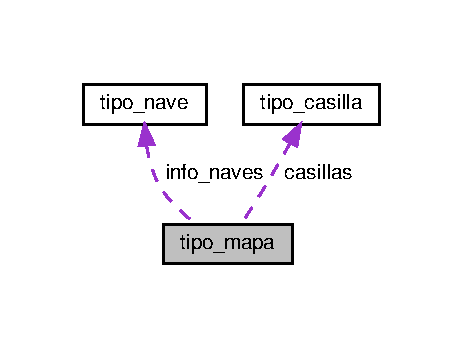
\includegraphics[width=222pt]{structtipo__mapa__coll__graph}
\end{center}
\end{figure}
\subsection*{Atributos públicos}
\begin{DoxyCompactItemize}
\item 
\mbox{\Hypertarget{structtipo__mapa_a4796e19ff6b789ec44086b1bd662cd37}\label{structtipo__mapa_a4796e19ff6b789ec44086b1bd662cd37}} 
\hyperlink{structtipo__nave}{tipo\+\_\+nave} \hyperlink{structtipo__mapa_a4796e19ff6b789ec44086b1bd662cd37}{info\+\_\+naves} \mbox{[}\hyperlink{types_8h_ab306668933fb4316ac0f5ef291d13dff}{N\+\_\+\+E\+Q\+U\+I\+P\+OS}\mbox{]}\mbox{[}\hyperlink{types_8h_aa1f2aba814c6d46772f9694849eeaa7a}{N\+\_\+\+N\+A\+V\+ES}\mbox{]}
\begin{DoxyCompactList}\small\item\em Naves de cada equipo. \end{DoxyCompactList}\item 
\mbox{\Hypertarget{structtipo__mapa_a92396d1db1745ec9b6aa2e53adf8981e}\label{structtipo__mapa_a92396d1db1745ec9b6aa2e53adf8981e}} 
\hyperlink{structtipo__casilla}{tipo\+\_\+casilla} \hyperlink{structtipo__mapa_a92396d1db1745ec9b6aa2e53adf8981e}{casillas} \mbox{[}\hyperlink{types_8h_a3f33f475897a86ab01a06d506eb0d925}{M\+A\+P\+A\+\_\+\+M\+A\+X\+\_\+Y}\mbox{]}\mbox{[}\hyperlink{types_8h_aef2eccdd4c60af9c7f30ed4eb2a567b0}{M\+A\+P\+A\+\_\+\+M\+A\+X\+\_\+X}\mbox{]}
\begin{DoxyCompactList}\small\item\em Casillas que componen el mapa. \end{DoxyCompactList}\item 
\mbox{\Hypertarget{structtipo__mapa_a5a59bf5262122191c18e3a94eae24a8c}\label{structtipo__mapa_a5a59bf5262122191c18e3a94eae24a8c}} 
int \hyperlink{structtipo__mapa_a5a59bf5262122191c18e3a94eae24a8c}{num\+\_\+naves} \mbox{[}\hyperlink{types_8h_ab306668933fb4316ac0f5ef291d13dff}{N\+\_\+\+E\+Q\+U\+I\+P\+OS}\mbox{]}
\begin{DoxyCompactList}\small\item\em Número de naves vivas en un equipo. \end{DoxyCompactList}\end{DoxyCompactItemize}


La documentación para esta estructura fue generada a partir del siguiente fichero\+:\begin{DoxyCompactItemize}
\item 
src/\hyperlink{types_8h}{types.\+h}\end{DoxyCompactItemize}

\hypertarget{structtipo__nave}{}\section{Referencia de la Estructura tipo\+\_\+nave}
\label{structtipo__nave}\index{tipo\+\_\+nave@{tipo\+\_\+nave}}
\subsection*{Atributos públicos}
\begin{DoxyCompactItemize}
\item 
\mbox{\Hypertarget{structtipo__nave_a319f01d0152cadf2b976ef51c93ff7ae}\label{structtipo__nave_a319f01d0152cadf2b976ef51c93ff7ae}} 
int \hyperlink{structtipo__nave_a319f01d0152cadf2b976ef51c93ff7ae}{vida}
\begin{DoxyCompactList}\small\item\em Vida que le queda a la nave. \end{DoxyCompactList}\item 
\mbox{\Hypertarget{structtipo__nave_ae3a263a841c045b4de31b2e4a3838fc1}\label{structtipo__nave_ae3a263a841c045b4de31b2e4a3838fc1}} 
int \hyperlink{structtipo__nave_ae3a263a841c045b4de31b2e4a3838fc1}{pos\+\_\+x}
\begin{DoxyCompactList}\small\item\em Columna en el mapa. \end{DoxyCompactList}\item 
\mbox{\Hypertarget{structtipo__nave_a6c502ff05341d19b9f00c83730121bfe}\label{structtipo__nave_a6c502ff05341d19b9f00c83730121bfe}} 
int \hyperlink{structtipo__nave_a6c502ff05341d19b9f00c83730121bfe}{pos\+\_\+y}
\begin{DoxyCompactList}\small\item\em Fila en el mapa. \end{DoxyCompactList}\item 
\mbox{\Hypertarget{structtipo__nave_a9cef996f47c2096f5ee3752c26adde97}\label{structtipo__nave_a9cef996f47c2096f5ee3752c26adde97}} 
int \hyperlink{structtipo__nave_a9cef996f47c2096f5ee3752c26adde97}{equipo}
\begin{DoxyCompactList}\small\item\em Equipo de la nave. \end{DoxyCompactList}\item 
\mbox{\Hypertarget{structtipo__nave_a4e63a4af5631f52382dae374ef4f9760}\label{structtipo__nave_a4e63a4af5631f52382dae374ef4f9760}} 
int \hyperlink{structtipo__nave_a4e63a4af5631f52382dae374ef4f9760}{num\+\_\+nave}
\begin{DoxyCompactList}\small\item\em Numero de la nave en el equipo. \end{DoxyCompactList}\item 
\mbox{\Hypertarget{structtipo__nave_a5fd530b54ff7694b07d41d3a168b800c}\label{structtipo__nave_a5fd530b54ff7694b07d41d3a168b800c}} 
bool \hyperlink{structtipo__nave_a5fd530b54ff7694b07d41d3a168b800c}{viva}
\begin{DoxyCompactList}\small\item\em Si la nave está viva o ha sido destruida. \end{DoxyCompactList}\end{DoxyCompactItemize}


La documentación para esta estructura fue generada a partir del siguiente fichero\+:\begin{DoxyCompactItemize}
\item 
src/\hyperlink{types_8h}{types.\+h}\end{DoxyCompactItemize}

\chapter{Documentación de archivos}
\hypertarget{gamescreen_8c}{}\section{Referencia del Archivo src/gamescreen.c}
\label{gamescreen_8c}\index{src/gamescreen.\+c@{src/gamescreen.\+c}}


Código fuente del modo pantalla.  


{\ttfamily \#include $<$ncurses.\+h$>$}\newline
Dependencia gráfica adjunta para gamescreen.\+c\+:
\nopagebreak
\begin{figure}[H]
\begin{center}
\leavevmode
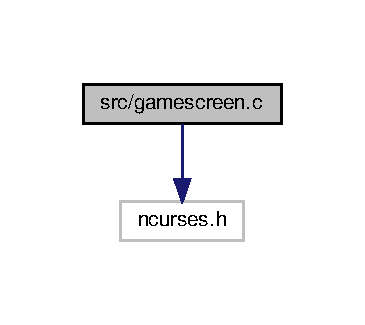
\includegraphics[width=175pt]{gamescreen_8c__incl}
\end{center}
\end{figure}
\subsection*{Funciones}
\begin{DoxyCompactItemize}
\item 
void \hyperlink{gamescreen_8c_a9dbb6c251337c03c078dc330caee48d2}{screen\+\_\+init} ()
\item 
void \hyperlink{gamescreen_8c_a0780ee70c58765ba78d2c686dd14bd78}{screen\+\_\+addch} (int row, int col, char symbol)
\item 
void \hyperlink{gamescreen_8c_ab866ab906055d0fb46f4ccfa07c82173}{screen\+\_\+refresh} ()
\item 
void \hyperlink{gamescreen_8c_af3bc8be95518f1d57d6d201a980359be}{screen\+\_\+end} ()
\end{DoxyCompactItemize}


\subsection{Descripción detallada}
Código fuente del modo pantalla. 



\subsection{Documentación de las funciones}
\mbox{\Hypertarget{gamescreen_8c_a0780ee70c58765ba78d2c686dd14bd78}\label{gamescreen_8c_a0780ee70c58765ba78d2c686dd14bd78}} 
\index{gamescreen.\+c@{gamescreen.\+c}!screen\+\_\+addch@{screen\+\_\+addch}}
\index{screen\+\_\+addch@{screen\+\_\+addch}!gamescreen.\+c@{gamescreen.\+c}}
\subsubsection{\texorpdfstring{screen\+\_\+addch()}{screen\_addch()}}
{\footnotesize\ttfamily void screen\+\_\+addch (\begin{DoxyParamCaption}\item[{int}]{row,  }\item[{int}]{col,  }\item[{char}]{symbol }\end{DoxyParamCaption})}

Fija en pantalla un símbolo en la posición (fila, columna). Siendo (0, 0) la esquina superior izquierda. El símbolo no se mostrará hasta el próximo \hyperlink{gamescreen_8c_ab866ab906055d0fb46f4ccfa07c82173}{screen\+\_\+refresh()}. 
\begin{DoxyParams}{Parámetros}
{\em row} & Fila a la que añadir el carácter especificado \\
\hline
{\em col} & Columna a la que añadir el carácter especificado \\
\hline
{\em symbol} & Símbolo a añadir \\
\hline
\end{DoxyParams}
\mbox{\Hypertarget{gamescreen_8c_af3bc8be95518f1d57d6d201a980359be}\label{gamescreen_8c_af3bc8be95518f1d57d6d201a980359be}} 
\index{gamescreen.\+c@{gamescreen.\+c}!screen\+\_\+end@{screen\+\_\+end}}
\index{screen\+\_\+end@{screen\+\_\+end}!gamescreen.\+c@{gamescreen.\+c}}
\subsubsection{\texorpdfstring{screen\+\_\+end()}{screen\_end()}}
{\footnotesize\ttfamily void screen\+\_\+end (\begin{DoxyParamCaption}{ }\end{DoxyParamCaption})}

Finaliza el modo pantalla. Hay que hacerlo antes de finalizar el programa. \mbox{\Hypertarget{gamescreen_8c_a9dbb6c251337c03c078dc330caee48d2}\label{gamescreen_8c_a9dbb6c251337c03c078dc330caee48d2}} 
\index{gamescreen.\+c@{gamescreen.\+c}!screen\+\_\+init@{screen\+\_\+init}}
\index{screen\+\_\+init@{screen\+\_\+init}!gamescreen.\+c@{gamescreen.\+c}}
\subsubsection{\texorpdfstring{screen\+\_\+init()}{screen\_init()}}
{\footnotesize\ttfamily void screen\+\_\+init (\begin{DoxyParamCaption}{ }\end{DoxyParamCaption})}

Inicializa el modo pantalla en el terminal. Debe hacerse antes que cualquier otra función screen. \mbox{\Hypertarget{gamescreen_8c_ab866ab906055d0fb46f4ccfa07c82173}\label{gamescreen_8c_ab866ab906055d0fb46f4ccfa07c82173}} 
\index{gamescreen.\+c@{gamescreen.\+c}!screen\+\_\+refresh@{screen\+\_\+refresh}}
\index{screen\+\_\+refresh@{screen\+\_\+refresh}!gamescreen.\+c@{gamescreen.\+c}}
\subsubsection{\texorpdfstring{screen\+\_\+refresh()}{screen\_refresh()}}
{\footnotesize\ttfamily void screen\+\_\+refresh (\begin{DoxyParamCaption}{ }\end{DoxyParamCaption})}

Refresca lo que muestra la pantalla. En principio, no hay que hacer refresh cada vez que se añade un símbolo con \hyperlink{gamescreen_8c_a0780ee70c58765ba78d2c686dd14bd78}{screen\+\_\+addch()}. 
\hypertarget{gamescreen_8h}{}\section{Referencia del Archivo src/gamescreen.h}
\label{gamescreen_8h}\index{src/gamescreen.\+h@{src/gamescreen.\+h}}


Cabecera del modo pantalla.  


Gráfico de los archivos que directa o indirectamente incluyen a este archivo\+:
\nopagebreak
\begin{figure}[H]
\begin{center}
\leavevmode
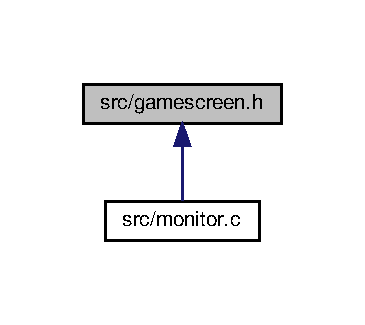
\includegraphics[width=175pt]{gamescreen_8h__dep__incl}
\end{center}
\end{figure}
\subsection*{Funciones}
\begin{DoxyCompactItemize}
\item 
void \hyperlink{gamescreen_8h_a9dbb6c251337c03c078dc330caee48d2}{screen\+\_\+init} ()
\item 
void \hyperlink{gamescreen_8h_a0780ee70c58765ba78d2c686dd14bd78}{screen\+\_\+addch} (int row, int col, char symbol)
\item 
void \hyperlink{gamescreen_8h_ab866ab906055d0fb46f4ccfa07c82173}{screen\+\_\+refresh} ()
\item 
void \hyperlink{gamescreen_8h_af3bc8be95518f1d57d6d201a980359be}{screen\+\_\+end} ()
\end{DoxyCompactItemize}


\subsection{Descripción detallada}
Cabecera del modo pantalla. 



\subsection{Documentación de las funciones}
\mbox{\Hypertarget{gamescreen_8h_a0780ee70c58765ba78d2c686dd14bd78}\label{gamescreen_8h_a0780ee70c58765ba78d2c686dd14bd78}} 
\index{gamescreen.\+h@{gamescreen.\+h}!screen\+\_\+addch@{screen\+\_\+addch}}
\index{screen\+\_\+addch@{screen\+\_\+addch}!gamescreen.\+h@{gamescreen.\+h}}
\subsubsection{\texorpdfstring{screen\+\_\+addch()}{screen\_addch()}}
{\footnotesize\ttfamily void screen\+\_\+addch (\begin{DoxyParamCaption}\item[{int}]{row,  }\item[{int}]{col,  }\item[{char}]{symbol }\end{DoxyParamCaption})}

Fija en pantalla un símbolo en la posición (fila, columna). Siendo (0, 0) la esquina superior izquierda. El símbolo no se mostrará hasta el próximo \hyperlink{gamescreen_8h_ab866ab906055d0fb46f4ccfa07c82173}{screen\+\_\+refresh()}. 
\begin{DoxyParams}{Parámetros}
{\em row} & Fila a la que añadir el carácter especificado \\
\hline
{\em col} & Columna a la que añadir el carácter especificado \\
\hline
{\em symbol} & Símbolo a añadir \\
\hline
\end{DoxyParams}
\mbox{\Hypertarget{gamescreen_8h_af3bc8be95518f1d57d6d201a980359be}\label{gamescreen_8h_af3bc8be95518f1d57d6d201a980359be}} 
\index{gamescreen.\+h@{gamescreen.\+h}!screen\+\_\+end@{screen\+\_\+end}}
\index{screen\+\_\+end@{screen\+\_\+end}!gamescreen.\+h@{gamescreen.\+h}}
\subsubsection{\texorpdfstring{screen\+\_\+end()}{screen\_end()}}
{\footnotesize\ttfamily void screen\+\_\+end (\begin{DoxyParamCaption}{ }\end{DoxyParamCaption})}

Finaliza el modo pantalla. Hay que hacerlo antes de finalizar el programa. \mbox{\Hypertarget{gamescreen_8h_a9dbb6c251337c03c078dc330caee48d2}\label{gamescreen_8h_a9dbb6c251337c03c078dc330caee48d2}} 
\index{gamescreen.\+h@{gamescreen.\+h}!screen\+\_\+init@{screen\+\_\+init}}
\index{screen\+\_\+init@{screen\+\_\+init}!gamescreen.\+h@{gamescreen.\+h}}
\subsubsection{\texorpdfstring{screen\+\_\+init()}{screen\_init()}}
{\footnotesize\ttfamily void screen\+\_\+init (\begin{DoxyParamCaption}{ }\end{DoxyParamCaption})}

Inicializa el modo pantalla en el terminal. Debe hacerse antes que cualquier otra función screen. \mbox{\Hypertarget{gamescreen_8h_ab866ab906055d0fb46f4ccfa07c82173}\label{gamescreen_8h_ab866ab906055d0fb46f4ccfa07c82173}} 
\index{gamescreen.\+h@{gamescreen.\+h}!screen\+\_\+refresh@{screen\+\_\+refresh}}
\index{screen\+\_\+refresh@{screen\+\_\+refresh}!gamescreen.\+h@{gamescreen.\+h}}
\subsubsection{\texorpdfstring{screen\+\_\+refresh()}{screen\_refresh()}}
{\footnotesize\ttfamily void screen\+\_\+refresh (\begin{DoxyParamCaption}{ }\end{DoxyParamCaption})}

Refresca lo que muestra la pantalla. En principio, no hay que hacer refresh cada vez que se añade un símbolo con \hyperlink{gamescreen_8h_a0780ee70c58765ba78d2c686dd14bd78}{screen\+\_\+addch()}. 
\hypertarget{jefe_8c}{}\section{Referencia del Archivo src/jefe.c}
\label{jefe_8c}\index{src/jefe.\+c@{src/jefe.\+c}}


Código fuente de jefe.  


{\ttfamily \#include \char`\"{}jefe.\+h\char`\"{}}\newline
Dependencia gráfica adjunta para jefe.\+c\+:
\nopagebreak
\begin{figure}[H]
\begin{center}
\leavevmode
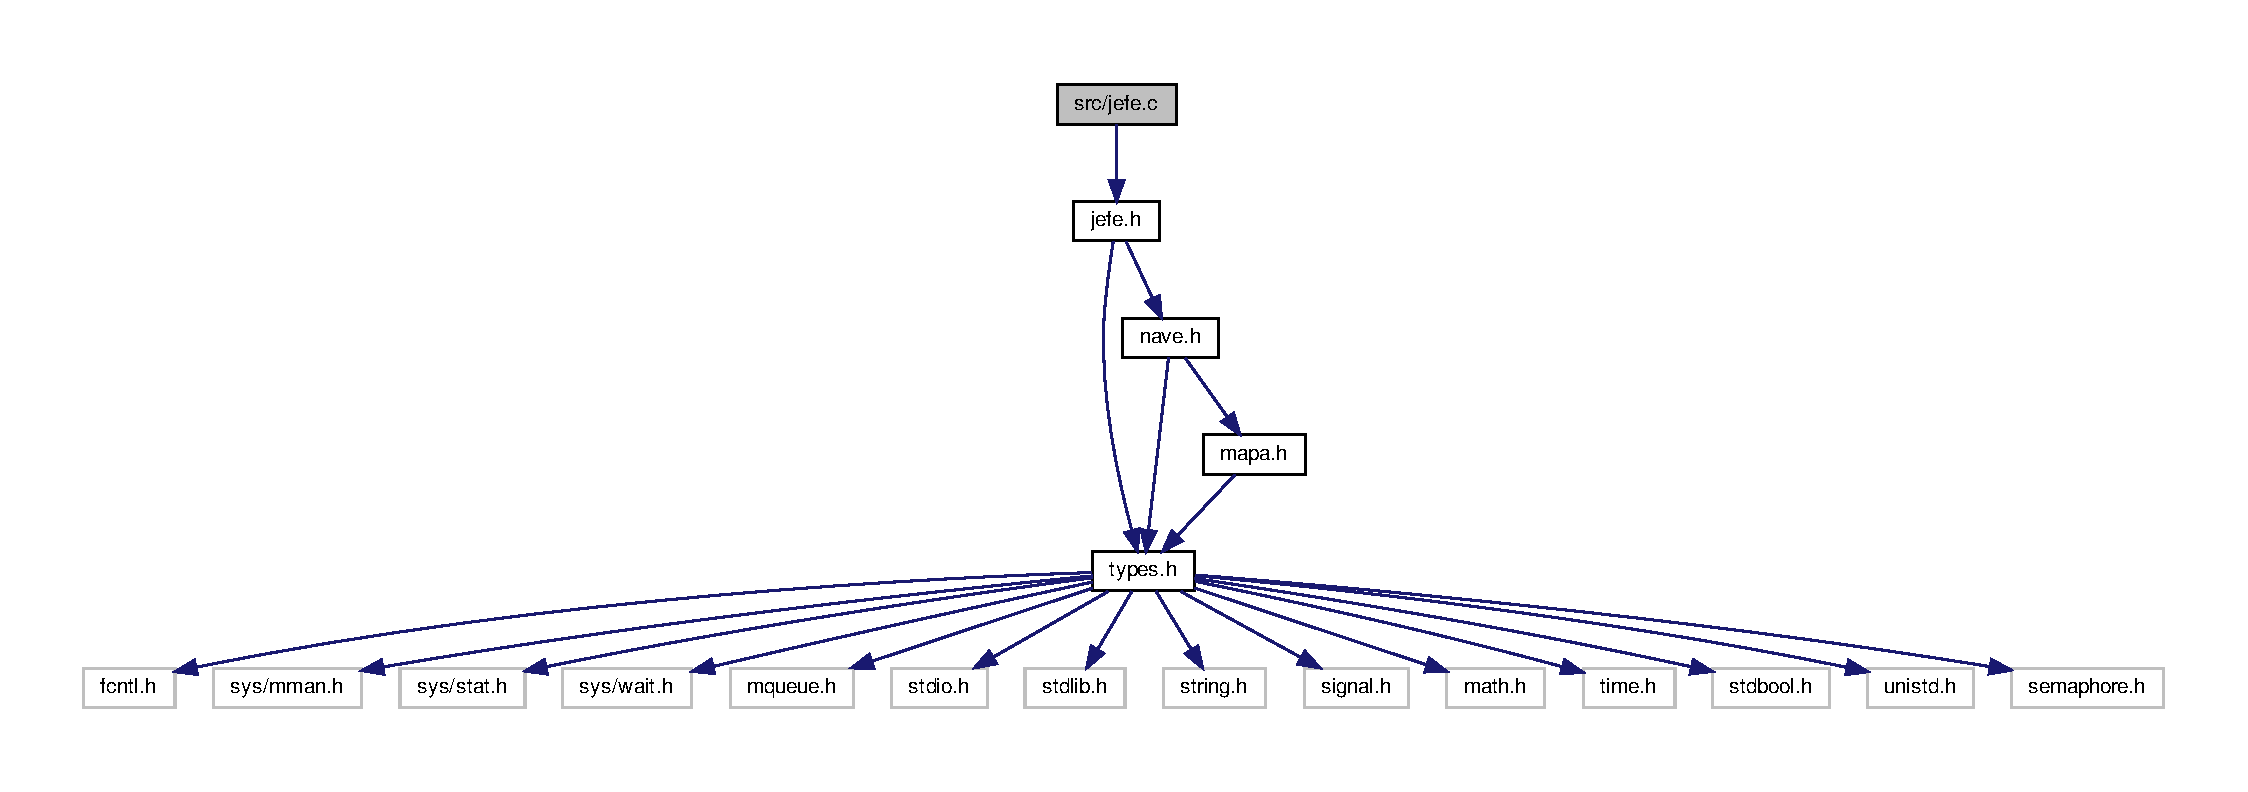
\includegraphics[width=350pt]{jefe_8c__incl}
\end{center}
\end{figure}
\subsection*{Funciones}
\begin{DoxyCompactItemize}
\item 
void \hyperlink{jefe_8c_a7cce1e5586fbabeb1af35fc7de5b2bfc}{jefe\+\_\+crear\+\_\+naves} (\hyperlink{structtipo__mapa}{tipo\+\_\+mapa} $\ast$mapa, int n\+\_\+equipo, int fd\+\_\+jefe\mbox{[}\hyperlink{types_8h_aa1f2aba814c6d46772f9694849eeaa7a}{N\+\_\+\+N\+A\+V\+ES}\mbox{]}\mbox{[}2\mbox{]}, pid\+\_\+t pids\+\_\+naves\mbox{[}\hyperlink{types_8h_aa1f2aba814c6d46772f9694849eeaa7a}{N\+\_\+\+N\+A\+V\+ES}\mbox{]})
\item 
void \hyperlink{jefe_8c_acc2874834095a0921d3b644130bfb4c6}{jefe} (\hyperlink{structtipo__mapa}{tipo\+\_\+mapa} $\ast$mapa, int n\+\_\+equipo, int fd\+\_\+sim\mbox{[}2\mbox{]}, sem\+\_\+t $\ast$sem\+\_\+equipos\+\_\+listos)
\end{DoxyCompactItemize}


\subsection{Descripción detallada}
Código fuente de jefe. 



\subsection{Documentación de las funciones}
\mbox{\Hypertarget{jefe_8c_acc2874834095a0921d3b644130bfb4c6}\label{jefe_8c_acc2874834095a0921d3b644130bfb4c6}} 
\index{jefe.\+c@{jefe.\+c}!jefe@{jefe}}
\index{jefe@{jefe}!jefe.\+c@{jefe.\+c}}
\subsubsection{\texorpdfstring{jefe()}{jefe()}}
{\footnotesize\ttfamily void jefe (\begin{DoxyParamCaption}\item[{\hyperlink{structtipo__mapa}{tipo\+\_\+mapa} $\ast$}]{mapa,  }\item[{int}]{n\+\_\+equipo,  }\item[{int}]{fd\+\_\+sim\mbox{[}2\mbox{]},  }\item[{sem\+\_\+t $\ast$}]{sem\+\_\+equipos\+\_\+listos }\end{DoxyParamCaption})}

Emula el comportamiento de un jefe. Se ocupa de crear los procesos nave y de mandarles órdenes de acción en cada turno. Gestiona la comunicación entre el simulador y las naves. 
\begin{DoxyParams}{Parámetros}
{\em mapa} & Puntero al mapa sobre el que debe trabajar el jefe \\
\hline
{\em n\+\_\+equipo} & Número de equipo del jefe \\
\hline
{\em fd\+\_\+sim} & Pipe que le permite comunicarse con el simulador \\
\hline
{\em sem\+\_\+equipos\+\_\+listos} & Semáforo que permite al simulador saber cúando estan listos los jefes \\
\hline
\end{DoxyParams}
\begin{DoxySeeAlso}{Ver también}
\hyperlink{nave_8c_a3d3f3f9b58aa6d6db95e19023d33f163}{nave()} 

\hyperlink{simulador_8c_a7ca1584ef7c92847d2a610dffac0ccba}{simulador()} 
\end{DoxySeeAlso}
\mbox{\Hypertarget{jefe_8c_a7cce1e5586fbabeb1af35fc7de5b2bfc}\label{jefe_8c_a7cce1e5586fbabeb1af35fc7de5b2bfc}} 
\index{jefe.\+c@{jefe.\+c}!jefe\+\_\+crear\+\_\+naves@{jefe\+\_\+crear\+\_\+naves}}
\index{jefe\+\_\+crear\+\_\+naves@{jefe\+\_\+crear\+\_\+naves}!jefe.\+c@{jefe.\+c}}
\subsubsection{\texorpdfstring{jefe\+\_\+crear\+\_\+naves()}{jefe\_crear\_naves()}}
{\footnotesize\ttfamily void jefe\+\_\+crear\+\_\+naves (\begin{DoxyParamCaption}\item[{\hyperlink{structtipo__mapa}{tipo\+\_\+mapa} $\ast$}]{mapa,  }\item[{int}]{n\+\_\+equipo,  }\item[{int}]{fd\+\_\+jefe\mbox{[}\+N\+\_\+\+N\+A\+V\+E\+S\mbox{]}\mbox{[}2\mbox{]},  }\item[{pid\+\_\+t}]{pids\+\_\+naves\mbox{[}\+N\+\_\+\+N\+A\+V\+E\+S\mbox{]} }\end{DoxyParamCaption})}

Crea las naves del jefe y las conexiones entre las naves y el jefe. 
\begin{DoxyParams}{Parámetros}
{\em mapa} & Puntero al mapa sobre el que trabajan el jefe y las naves \\
\hline
{\em n\+\_\+equipo} & Número de equipo del jefe y las naves \\
\hline
{\em fd\+\_\+jefe} & Pipes que conectarán al jefe con sus naves \\
\hline
{\em pids\+\_\+naves} & En esta estructura se almacenarán los P\+I\+Ds de las naves que se creen \\
\hline
\end{DoxyParams}

\hypertarget{jefe_8h}{}\section{Referencia del Archivo src/jefe.h}
\label{jefe_8h}\index{src/jefe.\+h@{src/jefe.\+h}}


Recoge la funcionalidad de un jefe.  


{\ttfamily \#include \char`\"{}types.\+h\char`\"{}}\newline
{\ttfamily \#include \char`\"{}nave.\+h\char`\"{}}\newline
Dependencia gráfica adjunta para jefe.\+h\+:
\nopagebreak
\begin{figure}[H]
\begin{center}
\leavevmode
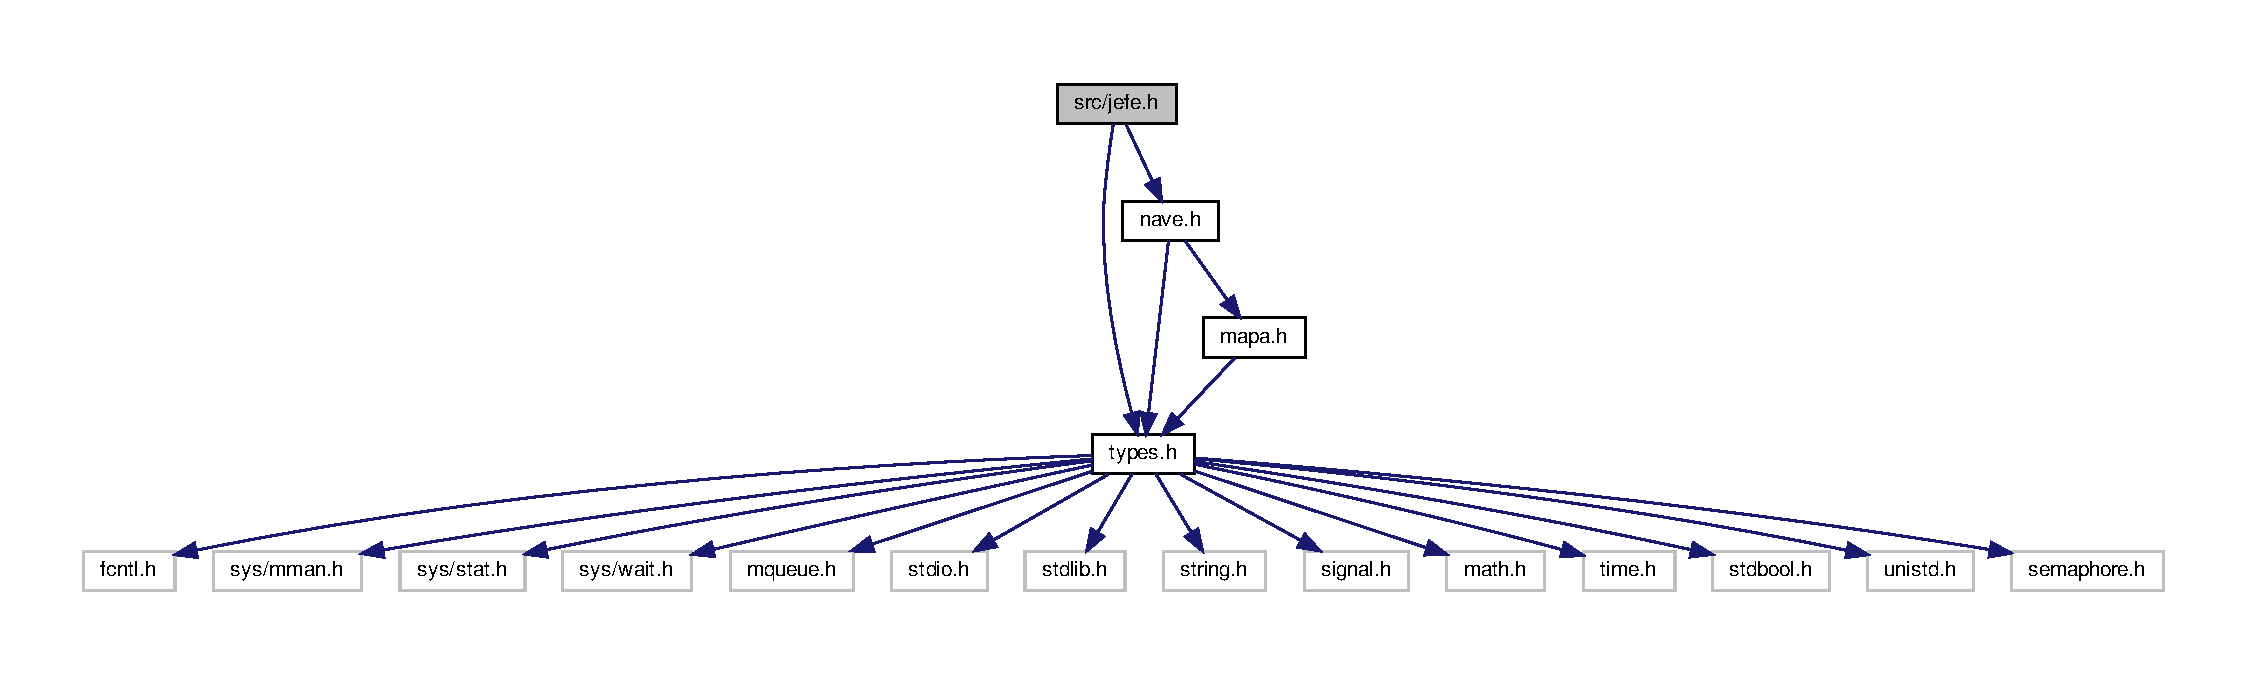
\includegraphics[width=350pt]{jefe_8h__incl}
\end{center}
\end{figure}
Gráfico de los archivos que directa o indirectamente incluyen a este archivo\+:
\nopagebreak
\begin{figure}[H]
\begin{center}
\leavevmode
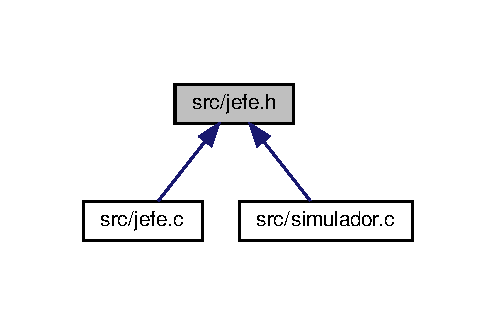
\includegraphics[width=238pt]{jefe_8h__dep__incl}
\end{center}
\end{figure}
\subsection*{Funciones}
\begin{DoxyCompactItemize}
\item 
void \hyperlink{jefe_8h_a1da6c9adb36fdd08899e9f54e06a0885}{jefe} (\hyperlink{structtipo__mapa}{tipo\+\_\+mapa} $\ast$mapa, int n\+\_\+equipo, int fd\+\_\+sim\mbox{[}2\mbox{]}, sem\+\_\+t $\ast$equipos\+\_\+listos)
\end{DoxyCompactItemize}


\subsection{Descripción detallada}
Recoge la funcionalidad de un jefe. 



\subsection{Documentación de las funciones}
\mbox{\Hypertarget{jefe_8h_a1da6c9adb36fdd08899e9f54e06a0885}\label{jefe_8h_a1da6c9adb36fdd08899e9f54e06a0885}} 
\index{jefe.\+h@{jefe.\+h}!jefe@{jefe}}
\index{jefe@{jefe}!jefe.\+h@{jefe.\+h}}
\subsubsection{\texorpdfstring{jefe()}{jefe()}}
{\footnotesize\ttfamily void jefe (\begin{DoxyParamCaption}\item[{\hyperlink{structtipo__mapa}{tipo\+\_\+mapa} $\ast$}]{mapa,  }\item[{int}]{n\+\_\+equipo,  }\item[{int}]{fd\+\_\+sim\mbox{[}2\mbox{]},  }\item[{sem\+\_\+t $\ast$}]{sem\+\_\+equipos\+\_\+listos }\end{DoxyParamCaption})}

Función que emula el comportamiento de un jefe. Se ocupa de crear los procesos nave y de mandarles órdenes de acción en cada turno. Gestiona la comunicación entre el simulador y las naves. 
\begin{DoxyParams}{Parámetros}
{\em mapa} & Puntero al mapa sobre el que debe trabajar el jefe \\
\hline
{\em n\+\_\+equipo} & Número de equipo del jefe \\
\hline
{\em fd\+\_\+sim} & Pipe que le permite comunicarse con el simulador \\
\hline
{\em sem\+\_\+equipos\+\_\+listos} & Semáforo que permite al simulador saber cúando estan listos los jefes \\
\hline
\end{DoxyParams}
\begin{DoxySeeAlso}{Ver también}
\hyperlink{nave_8c_a3d3f3f9b58aa6d6db95e19023d33f163}{nave()} 

\hyperlink{simulador_8c_a7ca1584ef7c92847d2a610dffac0ccba}{simulador()}
\end{DoxySeeAlso}
Emula el comportamiento de un jefe. Se ocupa de crear los procesos nave y de mandarles órdenes de acción en cada turno. Gestiona la comunicación entre el simulador y las naves. 
\begin{DoxyParams}{Parámetros}
{\em mapa} & Puntero al mapa sobre el que debe trabajar el jefe \\
\hline
{\em n\+\_\+equipo} & Número de equipo del jefe \\
\hline
{\em fd\+\_\+sim} & Pipe que le permite comunicarse con el simulador \\
\hline
{\em sem\+\_\+equipos\+\_\+listos} & Semáforo que permite al simulador saber cúando estan listos los jefes \\
\hline
\end{DoxyParams}
\begin{DoxySeeAlso}{Ver también}
\hyperlink{nave_8c_a3d3f3f9b58aa6d6db95e19023d33f163}{nave()} 

\hyperlink{simulador_8c_a7ca1584ef7c92847d2a610dffac0ccba}{simulador()} 
\end{DoxySeeAlso}

\hypertarget{mapa_8c}{}\section{Referencia del Archivo src/mapa.c}
\label{mapa_8c}\index{src/mapa.\+c@{src/mapa.\+c}}


Código fuente del mapa.  


{\ttfamily \#include \char`\"{}mapa.\+h\char`\"{}}\newline
Dependencia gráfica adjunta para mapa.\+c\+:
\nopagebreak
\begin{figure}[H]
\begin{center}
\leavevmode
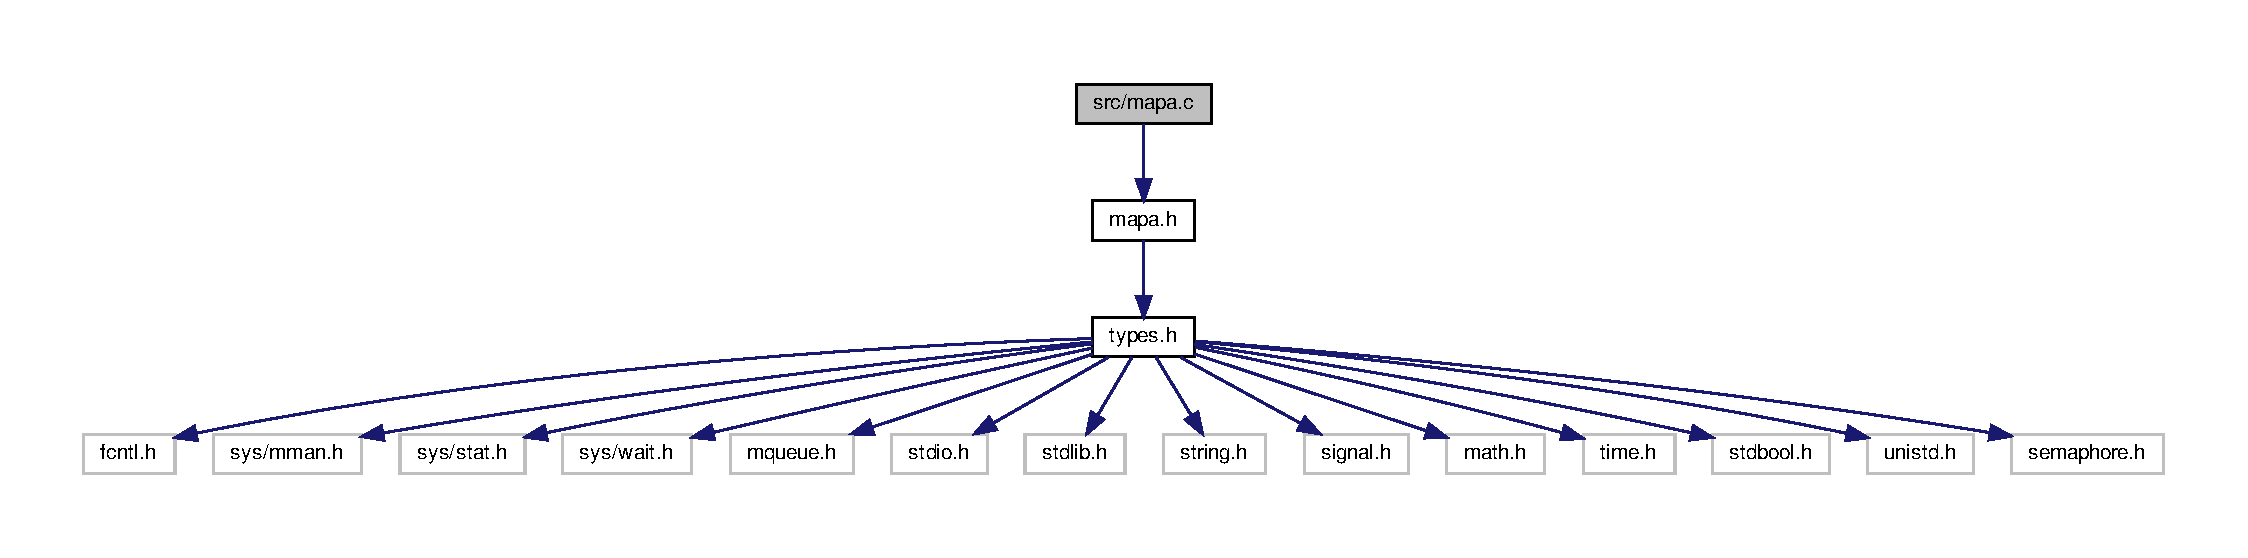
\includegraphics[width=350pt]{mapa_8c__incl}
\end{center}
\end{figure}
\subsection*{Funciones}
\begin{DoxyCompactItemize}
\item 
int \hyperlink{mapa_8c_a806dc48308c61c06fe9c5c5783bfad8d}{mapa\+\_\+clean\+\_\+casilla} (\hyperlink{structtipo__mapa}{tipo\+\_\+mapa} $\ast$mapa, int pos\+\_\+y, int pos\+\_\+x)
\item 
\hyperlink{structtipo__casilla}{tipo\+\_\+casilla} \hyperlink{mapa_8c_afd6289093c6647fc8feea1c01128cef8}{mapa\+\_\+get\+\_\+casilla} (\hyperlink{structtipo__mapa}{tipo\+\_\+mapa} $\ast$mapa, int pos\+\_\+y, int pos\+\_\+x)
\item 
int \hyperlink{mapa_8c_a85ae5ebedb02f18ac5a9c0d9296b20e9}{mapa\+\_\+get\+\_\+distancia} (\hyperlink{structtipo__mapa}{tipo\+\_\+mapa} $\ast$mapa, int ori\+\_\+y, int ori\+\_\+x, int target\+\_\+y, int target\+\_\+x)
\item 
\hyperlink{structtipo__nave}{tipo\+\_\+nave} \hyperlink{mapa_8c_ae949a08280aeec8b57b32906b6d73f78}{mapa\+\_\+get\+\_\+nave} (\hyperlink{structtipo__mapa}{tipo\+\_\+mapa} $\ast$mapa, int equipo, int num\+\_\+nave)
\item 
int \hyperlink{mapa_8c_a407e4361ece24cdd19cb0070181fbb91}{mapa\+\_\+get\+\_\+num\+\_\+naves} (\hyperlink{structtipo__mapa}{tipo\+\_\+mapa} $\ast$mapa, int equipo)
\item 
char \hyperlink{mapa_8c_a857fce0818018532b801cd6d4df10545}{mapa\+\_\+get\+\_\+symbol} (\hyperlink{structtipo__mapa}{tipo\+\_\+mapa} $\ast$mapa, int pos\+\_\+y, int pos\+\_\+x)
\item 
bool \hyperlink{mapa_8c_a67d3dfd58bcde49ba39a670eda876ae0}{mapa\+\_\+is\+\_\+casilla\+\_\+vacia} (\hyperlink{structtipo__mapa}{tipo\+\_\+mapa} $\ast$mapa, int pos\+\_\+y, int pos\+\_\+x)
\item 
void \hyperlink{mapa_8c_a555fccad30331311a6185a03c4a53f64}{mapa\+\_\+restore} (\hyperlink{structtipo__mapa}{tipo\+\_\+mapa} $\ast$mapa)
\item 
void \hyperlink{mapa_8c_ae732477c8a019a0c48fbc6cb65874b49}{mapa\+\_\+set\+\_\+symbol} (\hyperlink{structtipo__mapa}{tipo\+\_\+mapa} $\ast$mapa, int pos\+\_\+y, int pos\+\_\+x, char symbol)
\item 
int \hyperlink{mapa_8c_a9ffafdce1656b32f99897e5395cf3e04}{mapa\+\_\+set\+\_\+nave} (\hyperlink{structtipo__mapa}{tipo\+\_\+mapa} $\ast$mapa, \hyperlink{structtipo__nave}{tipo\+\_\+nave} \hyperlink{nave_8h_a3d3f3f9b58aa6d6db95e19023d33f163}{nave})
\item 
void \hyperlink{mapa_8c_a3a2e26d647b360f3cdf093a03ee15b79}{mapa\+\_\+set\+\_\+num\+\_\+naves} (\hyperlink{structtipo__mapa}{tipo\+\_\+mapa} $\ast$mapa, int equipo, int num\+\_\+naves)
\item 
void \hyperlink{mapa_8c_a70be4283077b695807f0e4448e13df0e}{mapa\+\_\+send\+\_\+misil} (\hyperlink{structtipo__mapa}{tipo\+\_\+mapa} $\ast$mapa, int origen\+\_\+y, int origen\+\_\+x, int target\+\_\+y, int target\+\_\+x)
\end{DoxyCompactItemize}
\subsection*{Variables}
\begin{DoxyCompactItemize}
\item 
\mbox{\Hypertarget{mapa_8c_a8aa1e6a79521de10e22a0a7574f2c8a5}\label{mapa_8c_a8aa1e6a79521de10e22a0a7574f2c8a5}} 
char \hyperlink{mapa_8c_a8aa1e6a79521de10e22a0a7574f2c8a5}{symbol\+\_\+equipos} \mbox{[}\hyperlink{types_8h_ab306668933fb4316ac0f5ef291d13dff}{N\+\_\+\+E\+Q\+U\+I\+P\+OS}\mbox{]} = \{\textquotesingle{}A\textquotesingle{}, \textquotesingle{}B\textquotesingle{}, \textquotesingle{}C\textquotesingle{}, \textquotesingle{}D\textquotesingle{}\}
\begin{DoxyCompactList}\small\item\em Símbolos de los diferentes equipos en el mapa (\hyperlink{mapa_8c}{mapa.\+c}) \end{DoxyCompactList}\end{DoxyCompactItemize}


\subsection{Descripción detallada}
Código fuente del mapa. 



\subsection{Documentación de las funciones}
\mbox{\Hypertarget{mapa_8c_a806dc48308c61c06fe9c5c5783bfad8d}\label{mapa_8c_a806dc48308c61c06fe9c5c5783bfad8d}} 
\index{mapa.\+c@{mapa.\+c}!mapa\+\_\+clean\+\_\+casilla@{mapa\+\_\+clean\+\_\+casilla}}
\index{mapa\+\_\+clean\+\_\+casilla@{mapa\+\_\+clean\+\_\+casilla}!mapa.\+c@{mapa.\+c}}
\subsubsection{\texorpdfstring{mapa\+\_\+clean\+\_\+casilla()}{mapa\_clean\_casilla()}}
{\footnotesize\ttfamily int mapa\+\_\+clean\+\_\+casilla (\begin{DoxyParamCaption}\item[{\hyperlink{structtipo__mapa}{tipo\+\_\+mapa} $\ast$}]{mapa,  }\item[{int}]{pos\+\_\+y,  }\item[{int}]{pos\+\_\+x }\end{DoxyParamCaption})}

Reinicia la casilla especificada. 
\begin{DoxyParams}{Parámetros}
{\em mapa} & Mapa de la simulación \\
\hline
{\em pos\+\_\+y} & Coordenada y de la casilla \\
\hline
{\em pos\+\_\+x} & Coordenada x de la casilla \\
\hline
\end{DoxyParams}
\begin{DoxyReturn}{Devuelve}
Devuelve 0 
\end{DoxyReturn}
\mbox{\Hypertarget{mapa_8c_afd6289093c6647fc8feea1c01128cef8}\label{mapa_8c_afd6289093c6647fc8feea1c01128cef8}} 
\index{mapa.\+c@{mapa.\+c}!mapa\+\_\+get\+\_\+casilla@{mapa\+\_\+get\+\_\+casilla}}
\index{mapa\+\_\+get\+\_\+casilla@{mapa\+\_\+get\+\_\+casilla}!mapa.\+c@{mapa.\+c}}
\subsubsection{\texorpdfstring{mapa\+\_\+get\+\_\+casilla()}{mapa\_get\_casilla()}}
{\footnotesize\ttfamily \hyperlink{structtipo__casilla}{tipo\+\_\+casilla} mapa\+\_\+get\+\_\+casilla (\begin{DoxyParamCaption}\item[{\hyperlink{structtipo__mapa}{tipo\+\_\+mapa} $\ast$}]{mapa,  }\item[{int}]{pos\+\_\+y,  }\item[{int}]{pos\+\_\+x }\end{DoxyParamCaption})}

Obtiene la casilla especificada. 
\begin{DoxyParams}{Parámetros}
{\em mapa} & Mapa de la simulación \\
\hline
{\em pos\+\_\+y} & Coordenada y de la casilla \\
\hline
{\em pos\+\_\+x} & Coordenada x de la casilla \\
\hline
\end{DoxyParams}
\begin{DoxyReturn}{Devuelve}
La casilla especificada. 
\end{DoxyReturn}
\mbox{\Hypertarget{mapa_8c_a85ae5ebedb02f18ac5a9c0d9296b20e9}\label{mapa_8c_a85ae5ebedb02f18ac5a9c0d9296b20e9}} 
\index{mapa.\+c@{mapa.\+c}!mapa\+\_\+get\+\_\+distancia@{mapa\+\_\+get\+\_\+distancia}}
\index{mapa\+\_\+get\+\_\+distancia@{mapa\+\_\+get\+\_\+distancia}!mapa.\+c@{mapa.\+c}}
\subsubsection{\texorpdfstring{mapa\+\_\+get\+\_\+distancia()}{mapa\_get\_distancia()}}
{\footnotesize\ttfamily int mapa\+\_\+get\+\_\+distancia (\begin{DoxyParamCaption}\item[{\hyperlink{structtipo__mapa}{tipo\+\_\+mapa} $\ast$}]{mapa,  }\item[{int}]{ori\+\_\+y,  }\item[{int}]{ori\+\_\+x,  }\item[{int}]{target\+\_\+y,  }\item[{int}]{target\+\_\+x }\end{DoxyParamCaption})}

Obtiene la distancia de las coordenadas de origen a las coordenadas objetivo. 
\begin{DoxyParams}{Parámetros}
{\em mapa} & Mapa de la simulación \\
\hline
{\em ori\+\_\+y} & Coordenada y origen \\
\hline
{\em ori\+\_\+x} & Coordenada x origen \\
\hline
{\em target\+\_\+y} & Coordenada y objetivo \\
\hline
{\em targer\+\_\+x} & Coordenada x objetivo \\
\hline
\end{DoxyParams}
\begin{DoxyReturn}{Devuelve}
Valor máximo entre la distancia en el eje X y la distancia en el eje Y 
\end{DoxyReturn}
\mbox{\Hypertarget{mapa_8c_ae949a08280aeec8b57b32906b6d73f78}\label{mapa_8c_ae949a08280aeec8b57b32906b6d73f78}} 
\index{mapa.\+c@{mapa.\+c}!mapa\+\_\+get\+\_\+nave@{mapa\+\_\+get\+\_\+nave}}
\index{mapa\+\_\+get\+\_\+nave@{mapa\+\_\+get\+\_\+nave}!mapa.\+c@{mapa.\+c}}
\subsubsection{\texorpdfstring{mapa\+\_\+get\+\_\+nave()}{mapa\_get\_nave()}}
{\footnotesize\ttfamily \hyperlink{structtipo__nave}{tipo\+\_\+nave} mapa\+\_\+get\+\_\+nave (\begin{DoxyParamCaption}\item[{\hyperlink{structtipo__mapa}{tipo\+\_\+mapa} $\ast$}]{mapa,  }\item[{int}]{equipo,  }\item[{int}]{num\+\_\+nave }\end{DoxyParamCaption})}

Devuelve la nave especificada del equipo indicado. 
\begin{DoxyParams}{Parámetros}
{\em mapa} & Mapa de la simulación \\
\hline
{\em equipo} & Equipo de la nave a devolver \\
\hline
{\em num\+\_\+nave} & Número de la nave a devolver \\
\hline
\end{DoxyParams}
\begin{DoxyReturn}{Devuelve}
Nave especificada del equipo indicado. 
\end{DoxyReturn}
\mbox{\Hypertarget{mapa_8c_a407e4361ece24cdd19cb0070181fbb91}\label{mapa_8c_a407e4361ece24cdd19cb0070181fbb91}} 
\index{mapa.\+c@{mapa.\+c}!mapa\+\_\+get\+\_\+num\+\_\+naves@{mapa\+\_\+get\+\_\+num\+\_\+naves}}
\index{mapa\+\_\+get\+\_\+num\+\_\+naves@{mapa\+\_\+get\+\_\+num\+\_\+naves}!mapa.\+c@{mapa.\+c}}
\subsubsection{\texorpdfstring{mapa\+\_\+get\+\_\+num\+\_\+naves()}{mapa\_get\_num\_naves()}}
{\footnotesize\ttfamily int mapa\+\_\+get\+\_\+num\+\_\+naves (\begin{DoxyParamCaption}\item[{\hyperlink{structtipo__mapa}{tipo\+\_\+mapa} $\ast$}]{mapa,  }\item[{int}]{equipo }\end{DoxyParamCaption})}

Devuelve el número de naves restantes del equipo indicado. 
\begin{DoxyParams}{Parámetros}
{\em mapa} & Mapa de la simulación \\
\hline
{\em equipo} & Equipo del que se desean conocer las naves restantes \\
\hline
\end{DoxyParams}
\begin{DoxyReturn}{Devuelve}
Naves restantes del equipo indicado. 
\end{DoxyReturn}
\mbox{\Hypertarget{mapa_8c_a857fce0818018532b801cd6d4df10545}\label{mapa_8c_a857fce0818018532b801cd6d4df10545}} 
\index{mapa.\+c@{mapa.\+c}!mapa\+\_\+get\+\_\+symbol@{mapa\+\_\+get\+\_\+symbol}}
\index{mapa\+\_\+get\+\_\+symbol@{mapa\+\_\+get\+\_\+symbol}!mapa.\+c@{mapa.\+c}}
\subsubsection{\texorpdfstring{mapa\+\_\+get\+\_\+symbol()}{mapa\_get\_symbol()}}
{\footnotesize\ttfamily char mapa\+\_\+get\+\_\+symbol (\begin{DoxyParamCaption}\item[{\hyperlink{structtipo__mapa}{tipo\+\_\+mapa} $\ast$}]{mapa,  }\item[{int}]{pos\+\_\+y,  }\item[{int}]{pos\+\_\+x }\end{DoxyParamCaption})}

Devuelve el símbolo de la casilla especificada. 
\begin{DoxyParams}{Parámetros}
{\em mapa} & Mapa de la simulación \\
\hline
{\em pos\+\_\+y} & Coordenada y de la casilla \\
\hline
{\em pos\+\_\+x} & Coordenada x de la casilla \\
\hline
\end{DoxyParams}
\begin{DoxyReturn}{Devuelve}
Símbolo de la casilla especificada. 
\end{DoxyReturn}
\mbox{\Hypertarget{mapa_8c_a67d3dfd58bcde49ba39a670eda876ae0}\label{mapa_8c_a67d3dfd58bcde49ba39a670eda876ae0}} 
\index{mapa.\+c@{mapa.\+c}!mapa\+\_\+is\+\_\+casilla\+\_\+vacia@{mapa\+\_\+is\+\_\+casilla\+\_\+vacia}}
\index{mapa\+\_\+is\+\_\+casilla\+\_\+vacia@{mapa\+\_\+is\+\_\+casilla\+\_\+vacia}!mapa.\+c@{mapa.\+c}}
\subsubsection{\texorpdfstring{mapa\+\_\+is\+\_\+casilla\+\_\+vacia()}{mapa\_is\_casilla\_vacia()}}
{\footnotesize\ttfamily bool mapa\+\_\+is\+\_\+casilla\+\_\+vacia (\begin{DoxyParamCaption}\item[{\hyperlink{structtipo__mapa}{tipo\+\_\+mapa} $\ast$}]{mapa,  }\item[{int}]{pos\+\_\+y,  }\item[{int}]{pos\+\_\+x }\end{DoxyParamCaption})}

Indica si la casilla especificada está vacía. 
\begin{DoxyParams}{Parámetros}
{\em mapa} & Mapa de la simulación \\
\hline
{\em pos\+\_\+y} & Coordenada y de la casilla \\
\hline
{\em pos\+\_\+x} & Coordenada x de la casilla \\
\hline
\end{DoxyParams}
\begin{DoxyReturn}{Devuelve}
Si la casilla especificada está vacía o no. 
\end{DoxyReturn}
\mbox{\Hypertarget{mapa_8c_a555fccad30331311a6185a03c4a53f64}\label{mapa_8c_a555fccad30331311a6185a03c4a53f64}} 
\index{mapa.\+c@{mapa.\+c}!mapa\+\_\+restore@{mapa\+\_\+restore}}
\index{mapa\+\_\+restore@{mapa\+\_\+restore}!mapa.\+c@{mapa.\+c}}
\subsubsection{\texorpdfstring{mapa\+\_\+restore()}{mapa\_restore()}}
{\footnotesize\ttfamily void mapa\+\_\+restore (\begin{DoxyParamCaption}\item[{\hyperlink{structtipo__mapa}{tipo\+\_\+mapa} $\ast$}]{mapa }\end{DoxyParamCaption})}

Restaura los símbolos de las casillas del mapa, conservando solo las naves. 
\begin{DoxyParams}{Parámetros}
{\em mapa} & Mapa de la simulación \\
\hline
\end{DoxyParams}
\mbox{\Hypertarget{mapa_8c_a70be4283077b695807f0e4448e13df0e}\label{mapa_8c_a70be4283077b695807f0e4448e13df0e}} 
\index{mapa.\+c@{mapa.\+c}!mapa\+\_\+send\+\_\+misil@{mapa\+\_\+send\+\_\+misil}}
\index{mapa\+\_\+send\+\_\+misil@{mapa\+\_\+send\+\_\+misil}!mapa.\+c@{mapa.\+c}}
\subsubsection{\texorpdfstring{mapa\+\_\+send\+\_\+misil()}{mapa\_send\_misil()}}
{\footnotesize\ttfamily void mapa\+\_\+send\+\_\+misil (\begin{DoxyParamCaption}\item[{\hyperlink{structtipo__mapa}{tipo\+\_\+mapa} $\ast$}]{mapa,  }\item[{int}]{origen\+\_\+y,  }\item[{int}]{origen\+\_\+x,  }\item[{int}]{target\+\_\+y,  }\item[{int}]{target\+\_\+x }\end{DoxyParamCaption})}

Imprime por pantalla la animación de un misil dirigido desde las coordenadas de origen a las de destino. 
\begin{DoxyParams}{Parámetros}
{\em mapa} & Mapa de la simulación \\
\hline
{\em ori\+\_\+y} & Coordenada y origen \\
\hline
{\em ori\+\_\+x} & Coordenada x origen \\
\hline
{\em target\+\_\+y} & Coordenada y objetivo \\
\hline
{\em targer\+\_\+x} & Coordenada x objetivo \\
\hline
\end{DoxyParams}
\mbox{\Hypertarget{mapa_8c_a9ffafdce1656b32f99897e5395cf3e04}\label{mapa_8c_a9ffafdce1656b32f99897e5395cf3e04}} 
\index{mapa.\+c@{mapa.\+c}!mapa\+\_\+set\+\_\+nave@{mapa\+\_\+set\+\_\+nave}}
\index{mapa\+\_\+set\+\_\+nave@{mapa\+\_\+set\+\_\+nave}!mapa.\+c@{mapa.\+c}}
\subsubsection{\texorpdfstring{mapa\+\_\+set\+\_\+nave()}{mapa\_set\_nave()}}
{\footnotesize\ttfamily int mapa\+\_\+set\+\_\+nave (\begin{DoxyParamCaption}\item[{\hyperlink{structtipo__mapa}{tipo\+\_\+mapa} $\ast$}]{mapa,  }\item[{\hyperlink{structtipo__nave}{tipo\+\_\+nave}}]{nave }\end{DoxyParamCaption})}

Añade una nueva nave al mapa de la simulación. 
\begin{DoxyParams}{Parámetros}
{\em mapa} & Mapa de la simulación \\
\hline
{\em nave} & Nueva nave que añadir al mapa \\
\hline
\end{DoxyParams}
\begin{DoxyReturn}{Devuelve}
Devuelve 0 
\end{DoxyReturn}
\mbox{\Hypertarget{mapa_8c_a3a2e26d647b360f3cdf093a03ee15b79}\label{mapa_8c_a3a2e26d647b360f3cdf093a03ee15b79}} 
\index{mapa.\+c@{mapa.\+c}!mapa\+\_\+set\+\_\+num\+\_\+naves@{mapa\+\_\+set\+\_\+num\+\_\+naves}}
\index{mapa\+\_\+set\+\_\+num\+\_\+naves@{mapa\+\_\+set\+\_\+num\+\_\+naves}!mapa.\+c@{mapa.\+c}}
\subsubsection{\texorpdfstring{mapa\+\_\+set\+\_\+num\+\_\+naves()}{mapa\_set\_num\_naves()}}
{\footnotesize\ttfamily void mapa\+\_\+set\+\_\+num\+\_\+naves (\begin{DoxyParamCaption}\item[{\hyperlink{structtipo__mapa}{tipo\+\_\+mapa} $\ast$}]{mapa,  }\item[{int}]{equipo,  }\item[{int}]{num\+\_\+naves }\end{DoxyParamCaption})}

Establece el número de naves restantes de un equipo. 
\begin{DoxyParams}{Parámetros}
{\em mapa} & Mapa de la simulación \\
\hline
{\em equipo} & Equipo al que se establecerá el nuevo valor de naves restantes \\
\hline
{\em num\+\_\+naves} & Naves restantes del equipo especificado \\
\hline
\end{DoxyParams}
\mbox{\Hypertarget{mapa_8c_ae732477c8a019a0c48fbc6cb65874b49}\label{mapa_8c_ae732477c8a019a0c48fbc6cb65874b49}} 
\index{mapa.\+c@{mapa.\+c}!mapa\+\_\+set\+\_\+symbol@{mapa\+\_\+set\+\_\+symbol}}
\index{mapa\+\_\+set\+\_\+symbol@{mapa\+\_\+set\+\_\+symbol}!mapa.\+c@{mapa.\+c}}
\subsubsection{\texorpdfstring{mapa\+\_\+set\+\_\+symbol()}{mapa\_set\_symbol()}}
{\footnotesize\ttfamily void mapa\+\_\+set\+\_\+symbol (\begin{DoxyParamCaption}\item[{\hyperlink{structtipo__mapa}{tipo\+\_\+mapa} $\ast$}]{mapa,  }\item[{int}]{pos\+\_\+y,  }\item[{int}]{pos\+\_\+x,  }\item[{char}]{symbol }\end{DoxyParamCaption})}

Establece el símbolo de la casilla especificada. 
\begin{DoxyParams}{Parámetros}
{\em mapa} & Mapa de la simulación \\
\hline
{\em pos\+\_\+y} & Coordenada y de la casilla \\
\hline
{\em pos\+\_\+x} & Coordenada x de la casilla \\
\hline
{\em symbol} & Nuevo símbolo de la casilla especificada. \\
\hline
\end{DoxyParams}

\hypertarget{mapa_8h}{}\section{Referencia del Archivo src/mapa.h}
\label{mapa_8h}\index{src/mapa.\+h@{src/mapa.\+h}}


Cabecera del mapa.  


{\ttfamily \#include \char`\"{}types.\+h\char`\"{}}\newline
Dependencia gráfica adjunta para mapa.\+h\+:
\nopagebreak
\begin{figure}[H]
\begin{center}
\leavevmode
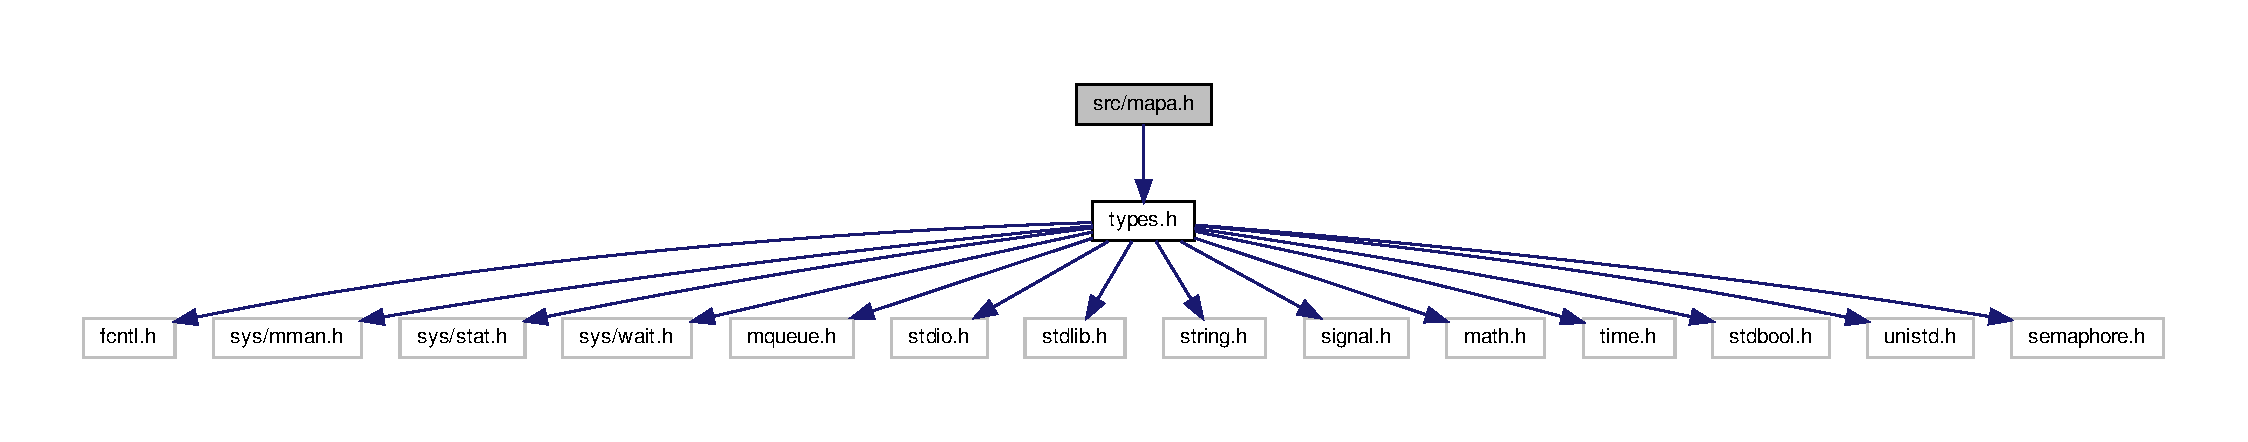
\includegraphics[width=350pt]{mapa_8h__incl}
\end{center}
\end{figure}
Gráfico de los archivos que directa o indirectamente incluyen a este archivo\+:
\nopagebreak
\begin{figure}[H]
\begin{center}
\leavevmode
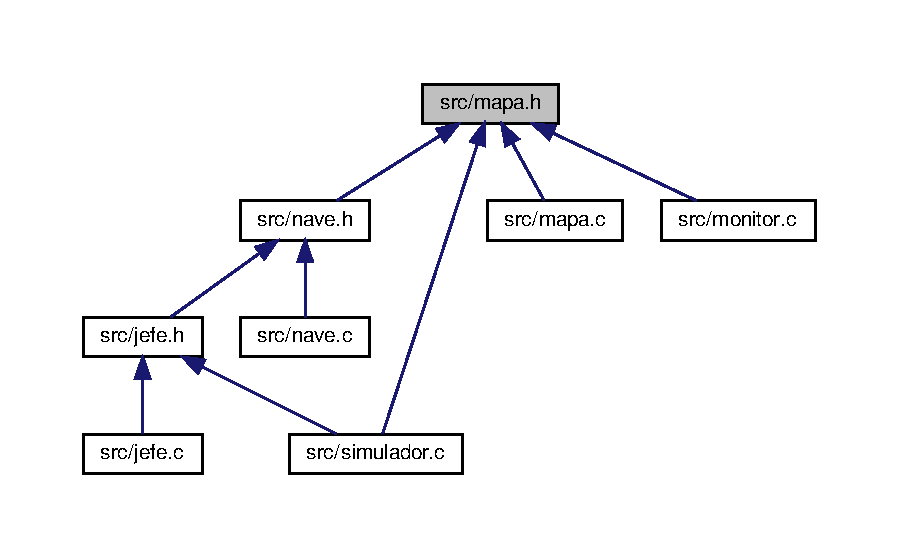
\includegraphics[width=350pt]{mapa_8h__dep__incl}
\end{center}
\end{figure}
\subsection*{Funciones}
\begin{DoxyCompactItemize}
\item 
int \hyperlink{mapa_8h_a806dc48308c61c06fe9c5c5783bfad8d}{mapa\+\_\+clean\+\_\+casilla} (\hyperlink{structtipo__mapa}{tipo\+\_\+mapa} $\ast$mapa, int pos\+\_\+y, int pos\+\_\+x)
\item 
\hyperlink{structtipo__casilla}{tipo\+\_\+casilla} \hyperlink{mapa_8h_adedc40364bffd27208a7287434c28c15}{mapa\+\_\+get\+\_\+casilla} (\hyperlink{structtipo__mapa}{tipo\+\_\+mapa} $\ast$mapa, int posy, int posx)
\item 
int \hyperlink{mapa_8h_a85ae5ebedb02f18ac5a9c0d9296b20e9}{mapa\+\_\+get\+\_\+distancia} (\hyperlink{structtipo__mapa}{tipo\+\_\+mapa} $\ast$mapa, int ori\+\_\+y, int ori\+\_\+x, int target\+\_\+y, int target\+\_\+x)
\item 
\hyperlink{structtipo__nave}{tipo\+\_\+nave} \hyperlink{mapa_8h_ae949a08280aeec8b57b32906b6d73f78}{mapa\+\_\+get\+\_\+nave} (\hyperlink{structtipo__mapa}{tipo\+\_\+mapa} $\ast$mapa, int equipo, int num\+\_\+nave)
\item 
int \hyperlink{mapa_8h_a407e4361ece24cdd19cb0070181fbb91}{mapa\+\_\+get\+\_\+num\+\_\+naves} (\hyperlink{structtipo__mapa}{tipo\+\_\+mapa} $\ast$mapa, int equipo)
\item 
char \hyperlink{mapa_8h_a857fce0818018532b801cd6d4df10545}{mapa\+\_\+get\+\_\+symbol} (\hyperlink{structtipo__mapa}{tipo\+\_\+mapa} $\ast$mapa, int pos\+\_\+y, int pos\+\_\+x)
\item 
bool \hyperlink{mapa_8h_a67d3dfd58bcde49ba39a670eda876ae0}{mapa\+\_\+is\+\_\+casilla\+\_\+vacia} (\hyperlink{structtipo__mapa}{tipo\+\_\+mapa} $\ast$mapa, int pos\+\_\+y, int pos\+\_\+x)
\item 
void \hyperlink{mapa_8h_a555fccad30331311a6185a03c4a53f64}{mapa\+\_\+restore} (\hyperlink{structtipo__mapa}{tipo\+\_\+mapa} $\ast$mapa)
\item 
void \hyperlink{mapa_8h_a70be4283077b695807f0e4448e13df0e}{mapa\+\_\+send\+\_\+misil} (\hyperlink{structtipo__mapa}{tipo\+\_\+mapa} $\ast$mapa, int origen\+\_\+y, int origen\+\_\+x, int target\+\_\+y, int target\+\_\+x)
\item 
int \hyperlink{mapa_8h_a9ffafdce1656b32f99897e5395cf3e04}{mapa\+\_\+set\+\_\+nave} (\hyperlink{structtipo__mapa}{tipo\+\_\+mapa} $\ast$mapa, \hyperlink{structtipo__nave}{tipo\+\_\+nave} \hyperlink{nave_8h_a3d3f3f9b58aa6d6db95e19023d33f163}{nave})
\item 
void \hyperlink{mapa_8h_a3a2e26d647b360f3cdf093a03ee15b79}{mapa\+\_\+set\+\_\+num\+\_\+naves} (\hyperlink{structtipo__mapa}{tipo\+\_\+mapa} $\ast$mapa, int equipo, int num\+\_\+naves)
\item 
void \hyperlink{mapa_8h_ae732477c8a019a0c48fbc6cb65874b49}{mapa\+\_\+set\+\_\+symbol} (\hyperlink{structtipo__mapa}{tipo\+\_\+mapa} $\ast$mapa, int pos\+\_\+y, int pos\+\_\+x, char symbol)
\end{DoxyCompactItemize}


\subsection{Descripción detallada}
Cabecera del mapa. 



\subsection{Documentación de las funciones}
\mbox{\Hypertarget{mapa_8h_a806dc48308c61c06fe9c5c5783bfad8d}\label{mapa_8h_a806dc48308c61c06fe9c5c5783bfad8d}} 
\index{mapa.\+h@{mapa.\+h}!mapa\+\_\+clean\+\_\+casilla@{mapa\+\_\+clean\+\_\+casilla}}
\index{mapa\+\_\+clean\+\_\+casilla@{mapa\+\_\+clean\+\_\+casilla}!mapa.\+h@{mapa.\+h}}
\subsubsection{\texorpdfstring{mapa\+\_\+clean\+\_\+casilla()}{mapa\_clean\_casilla()}}
{\footnotesize\ttfamily int mapa\+\_\+clean\+\_\+casilla (\begin{DoxyParamCaption}\item[{\hyperlink{structtipo__mapa}{tipo\+\_\+mapa} $\ast$}]{mapa,  }\item[{int}]{pos\+\_\+y,  }\item[{int}]{pos\+\_\+x }\end{DoxyParamCaption})}

Reinicia la casilla especificada. 
\begin{DoxyParams}{Parámetros}
{\em mapa} & Mapa de la simulación \\
\hline
{\em pos\+\_\+y} & Coordenada y de la casilla \\
\hline
{\em pos\+\_\+x} & Coordenada x de la casilla \\
\hline
\end{DoxyParams}
\begin{DoxyReturn}{Devuelve}
Devuelve 0 
\end{DoxyReturn}
\mbox{\Hypertarget{mapa_8h_adedc40364bffd27208a7287434c28c15}\label{mapa_8h_adedc40364bffd27208a7287434c28c15}} 
\index{mapa.\+h@{mapa.\+h}!mapa\+\_\+get\+\_\+casilla@{mapa\+\_\+get\+\_\+casilla}}
\index{mapa\+\_\+get\+\_\+casilla@{mapa\+\_\+get\+\_\+casilla}!mapa.\+h@{mapa.\+h}}
\subsubsection{\texorpdfstring{mapa\+\_\+get\+\_\+casilla()}{mapa\_get\_casilla()}}
{\footnotesize\ttfamily \hyperlink{structtipo__casilla}{tipo\+\_\+casilla} mapa\+\_\+get\+\_\+casilla (\begin{DoxyParamCaption}\item[{\hyperlink{structtipo__mapa}{tipo\+\_\+mapa} $\ast$}]{mapa,  }\item[{int}]{pos\+\_\+y,  }\item[{int}]{pos\+\_\+x }\end{DoxyParamCaption})}

Obtiene la casilla especificada. 
\begin{DoxyParams}{Parámetros}
{\em mapa} & Mapa de la simulación \\
\hline
{\em pos\+\_\+y} & Coordenada y de la casilla \\
\hline
{\em pos\+\_\+x} & Coordenada x de la casilla \\
\hline
\end{DoxyParams}
\begin{DoxyReturn}{Devuelve}
La casilla especificada. 
\end{DoxyReturn}
\mbox{\Hypertarget{mapa_8h_a85ae5ebedb02f18ac5a9c0d9296b20e9}\label{mapa_8h_a85ae5ebedb02f18ac5a9c0d9296b20e9}} 
\index{mapa.\+h@{mapa.\+h}!mapa\+\_\+get\+\_\+distancia@{mapa\+\_\+get\+\_\+distancia}}
\index{mapa\+\_\+get\+\_\+distancia@{mapa\+\_\+get\+\_\+distancia}!mapa.\+h@{mapa.\+h}}
\subsubsection{\texorpdfstring{mapa\+\_\+get\+\_\+distancia()}{mapa\_get\_distancia()}}
{\footnotesize\ttfamily int mapa\+\_\+get\+\_\+distancia (\begin{DoxyParamCaption}\item[{\hyperlink{structtipo__mapa}{tipo\+\_\+mapa} $\ast$}]{mapa,  }\item[{int}]{ori\+\_\+y,  }\item[{int}]{ori\+\_\+x,  }\item[{int}]{target\+\_\+y,  }\item[{int}]{target\+\_\+x }\end{DoxyParamCaption})}

Obtiene la distancia de las coordenadas de origen a las coordenadas objetivo. 
\begin{DoxyParams}{Parámetros}
{\em mapa} & Mapa de la simulación \\
\hline
{\em ori\+\_\+y} & Coordenada y origen \\
\hline
{\em ori\+\_\+x} & Coordenada x origen \\
\hline
{\em target\+\_\+y} & Coordenada y objetivo \\
\hline
{\em targer\+\_\+x} & Coordenada x objetivo \\
\hline
\end{DoxyParams}
\begin{DoxyReturn}{Devuelve}
Valor máximo entre la distancia en el eje X y la distancia en el eje Y 
\end{DoxyReturn}
\mbox{\Hypertarget{mapa_8h_ae949a08280aeec8b57b32906b6d73f78}\label{mapa_8h_ae949a08280aeec8b57b32906b6d73f78}} 
\index{mapa.\+h@{mapa.\+h}!mapa\+\_\+get\+\_\+nave@{mapa\+\_\+get\+\_\+nave}}
\index{mapa\+\_\+get\+\_\+nave@{mapa\+\_\+get\+\_\+nave}!mapa.\+h@{mapa.\+h}}
\subsubsection{\texorpdfstring{mapa\+\_\+get\+\_\+nave()}{mapa\_get\_nave()}}
{\footnotesize\ttfamily \hyperlink{structtipo__nave}{tipo\+\_\+nave} mapa\+\_\+get\+\_\+nave (\begin{DoxyParamCaption}\item[{\hyperlink{structtipo__mapa}{tipo\+\_\+mapa} $\ast$}]{mapa,  }\item[{int}]{equipo,  }\item[{int}]{num\+\_\+nave }\end{DoxyParamCaption})}

Devuelve la nave especificada del equipo indicado. 
\begin{DoxyParams}{Parámetros}
{\em mapa} & Mapa de la simulación \\
\hline
{\em equipo} & Equipo de la nave a devolver \\
\hline
{\em num\+\_\+nave} & Número de la nave a devolver \\
\hline
\end{DoxyParams}
\begin{DoxyReturn}{Devuelve}
Nave especificada del equipo indicado. 
\end{DoxyReturn}
\mbox{\Hypertarget{mapa_8h_a407e4361ece24cdd19cb0070181fbb91}\label{mapa_8h_a407e4361ece24cdd19cb0070181fbb91}} 
\index{mapa.\+h@{mapa.\+h}!mapa\+\_\+get\+\_\+num\+\_\+naves@{mapa\+\_\+get\+\_\+num\+\_\+naves}}
\index{mapa\+\_\+get\+\_\+num\+\_\+naves@{mapa\+\_\+get\+\_\+num\+\_\+naves}!mapa.\+h@{mapa.\+h}}
\subsubsection{\texorpdfstring{mapa\+\_\+get\+\_\+num\+\_\+naves()}{mapa\_get\_num\_naves()}}
{\footnotesize\ttfamily int mapa\+\_\+get\+\_\+num\+\_\+naves (\begin{DoxyParamCaption}\item[{\hyperlink{structtipo__mapa}{tipo\+\_\+mapa} $\ast$}]{mapa,  }\item[{int}]{equipo }\end{DoxyParamCaption})}

Devuelve el número de naves restantes del equipo indicado. 
\begin{DoxyParams}{Parámetros}
{\em mapa} & Mapa de la simulación \\
\hline
{\em equipo} & Equipo del que se desean conocer las naves restantes \\
\hline
\end{DoxyParams}
\begin{DoxyReturn}{Devuelve}
Naves restantes del equipo indicado. 
\end{DoxyReturn}
\mbox{\Hypertarget{mapa_8h_a857fce0818018532b801cd6d4df10545}\label{mapa_8h_a857fce0818018532b801cd6d4df10545}} 
\index{mapa.\+h@{mapa.\+h}!mapa\+\_\+get\+\_\+symbol@{mapa\+\_\+get\+\_\+symbol}}
\index{mapa\+\_\+get\+\_\+symbol@{mapa\+\_\+get\+\_\+symbol}!mapa.\+h@{mapa.\+h}}
\subsubsection{\texorpdfstring{mapa\+\_\+get\+\_\+symbol()}{mapa\_get\_symbol()}}
{\footnotesize\ttfamily char mapa\+\_\+get\+\_\+symbol (\begin{DoxyParamCaption}\item[{\hyperlink{structtipo__mapa}{tipo\+\_\+mapa} $\ast$}]{mapa,  }\item[{int}]{pos\+\_\+y,  }\item[{int}]{pos\+\_\+x }\end{DoxyParamCaption})}

Devuelve el símbolo de la casilla especificada. 
\begin{DoxyParams}{Parámetros}
{\em mapa} & Mapa de la simulación \\
\hline
{\em pos\+\_\+y} & Coordenada y de la casilla \\
\hline
{\em pos\+\_\+x} & Coordenada x de la casilla \\
\hline
\end{DoxyParams}
\begin{DoxyReturn}{Devuelve}
Símbolo de la casilla especificada. 
\end{DoxyReturn}
\mbox{\Hypertarget{mapa_8h_a67d3dfd58bcde49ba39a670eda876ae0}\label{mapa_8h_a67d3dfd58bcde49ba39a670eda876ae0}} 
\index{mapa.\+h@{mapa.\+h}!mapa\+\_\+is\+\_\+casilla\+\_\+vacia@{mapa\+\_\+is\+\_\+casilla\+\_\+vacia}}
\index{mapa\+\_\+is\+\_\+casilla\+\_\+vacia@{mapa\+\_\+is\+\_\+casilla\+\_\+vacia}!mapa.\+h@{mapa.\+h}}
\subsubsection{\texorpdfstring{mapa\+\_\+is\+\_\+casilla\+\_\+vacia()}{mapa\_is\_casilla\_vacia()}}
{\footnotesize\ttfamily bool mapa\+\_\+is\+\_\+casilla\+\_\+vacia (\begin{DoxyParamCaption}\item[{\hyperlink{structtipo__mapa}{tipo\+\_\+mapa} $\ast$}]{mapa,  }\item[{int}]{pos\+\_\+y,  }\item[{int}]{pos\+\_\+x }\end{DoxyParamCaption})}

Indica si la casilla especificada está vacía. 
\begin{DoxyParams}{Parámetros}
{\em mapa} & Mapa de la simulación \\
\hline
{\em pos\+\_\+y} & Coordenada y de la casilla \\
\hline
{\em pos\+\_\+x} & Coordenada x de la casilla \\
\hline
\end{DoxyParams}
\begin{DoxyReturn}{Devuelve}
Si la casilla especificada está vacía o no. 
\end{DoxyReturn}
\mbox{\Hypertarget{mapa_8h_a555fccad30331311a6185a03c4a53f64}\label{mapa_8h_a555fccad30331311a6185a03c4a53f64}} 
\index{mapa.\+h@{mapa.\+h}!mapa\+\_\+restore@{mapa\+\_\+restore}}
\index{mapa\+\_\+restore@{mapa\+\_\+restore}!mapa.\+h@{mapa.\+h}}
\subsubsection{\texorpdfstring{mapa\+\_\+restore()}{mapa\_restore()}}
{\footnotesize\ttfamily void mapa\+\_\+restore (\begin{DoxyParamCaption}\item[{\hyperlink{structtipo__mapa}{tipo\+\_\+mapa} $\ast$}]{mapa }\end{DoxyParamCaption})}

Restaura los símbolos de las casillas del mapa, conservando solo las naves. 
\begin{DoxyParams}{Parámetros}
{\em mapa} & Mapa de la simulación \\
\hline
\end{DoxyParams}
\mbox{\Hypertarget{mapa_8h_a70be4283077b695807f0e4448e13df0e}\label{mapa_8h_a70be4283077b695807f0e4448e13df0e}} 
\index{mapa.\+h@{mapa.\+h}!mapa\+\_\+send\+\_\+misil@{mapa\+\_\+send\+\_\+misil}}
\index{mapa\+\_\+send\+\_\+misil@{mapa\+\_\+send\+\_\+misil}!mapa.\+h@{mapa.\+h}}
\subsubsection{\texorpdfstring{mapa\+\_\+send\+\_\+misil()}{mapa\_send\_misil()}}
{\footnotesize\ttfamily void mapa\+\_\+send\+\_\+misil (\begin{DoxyParamCaption}\item[{\hyperlink{structtipo__mapa}{tipo\+\_\+mapa} $\ast$}]{mapa,  }\item[{int}]{origen\+\_\+y,  }\item[{int}]{origen\+\_\+x,  }\item[{int}]{target\+\_\+y,  }\item[{int}]{target\+\_\+x }\end{DoxyParamCaption})}

Establece el símbolo de la casilla especificada. 
\begin{DoxyParams}{Parámetros}
{\em mapa} & Mapa de la simulación \\
\hline
{\em pos\+\_\+y} & Coordenada y de la casilla \\
\hline
{\em pos\+\_\+x} & Coordenada x de la casilla \\
\hline
{\em symbol} & Nuevo símbolo de la casilla especificada.\\
\hline
\end{DoxyParams}
Imprime por pantalla la animación de un misil dirigido desde las coordenadas de origen a las de destino. 
\begin{DoxyParams}{Parámetros}
{\em mapa} & Mapa de la simulación \\
\hline
{\em ori\+\_\+y} & Coordenada y origen \\
\hline
{\em ori\+\_\+x} & Coordenada x origen \\
\hline
{\em target\+\_\+y} & Coordenada y objetivo \\
\hline
{\em targer\+\_\+x} & Coordenada x objetivo \\
\hline
\end{DoxyParams}
\mbox{\Hypertarget{mapa_8h_a9ffafdce1656b32f99897e5395cf3e04}\label{mapa_8h_a9ffafdce1656b32f99897e5395cf3e04}} 
\index{mapa.\+h@{mapa.\+h}!mapa\+\_\+set\+\_\+nave@{mapa\+\_\+set\+\_\+nave}}
\index{mapa\+\_\+set\+\_\+nave@{mapa\+\_\+set\+\_\+nave}!mapa.\+h@{mapa.\+h}}
\subsubsection{\texorpdfstring{mapa\+\_\+set\+\_\+nave()}{mapa\_set\_nave()}}
{\footnotesize\ttfamily int mapa\+\_\+set\+\_\+nave (\begin{DoxyParamCaption}\item[{\hyperlink{structtipo__mapa}{tipo\+\_\+mapa} $\ast$}]{mapa,  }\item[{\hyperlink{structtipo__nave}{tipo\+\_\+nave}}]{nave }\end{DoxyParamCaption})}

Añade una nueva nave al mapa de la simulación. 
\begin{DoxyParams}{Parámetros}
{\em mapa} & Mapa de la simulación \\
\hline
{\em nave} & Nueva nave que añadir al mapa \\
\hline
\end{DoxyParams}
\begin{DoxyReturn}{Devuelve}
Devuelve 0 
\end{DoxyReturn}
\mbox{\Hypertarget{mapa_8h_a3a2e26d647b360f3cdf093a03ee15b79}\label{mapa_8h_a3a2e26d647b360f3cdf093a03ee15b79}} 
\index{mapa.\+h@{mapa.\+h}!mapa\+\_\+set\+\_\+num\+\_\+naves@{mapa\+\_\+set\+\_\+num\+\_\+naves}}
\index{mapa\+\_\+set\+\_\+num\+\_\+naves@{mapa\+\_\+set\+\_\+num\+\_\+naves}!mapa.\+h@{mapa.\+h}}
\subsubsection{\texorpdfstring{mapa\+\_\+set\+\_\+num\+\_\+naves()}{mapa\_set\_num\_naves()}}
{\footnotesize\ttfamily void mapa\+\_\+set\+\_\+num\+\_\+naves (\begin{DoxyParamCaption}\item[{\hyperlink{structtipo__mapa}{tipo\+\_\+mapa} $\ast$}]{mapa,  }\item[{int}]{equipo,  }\item[{int}]{num\+\_\+naves }\end{DoxyParamCaption})}

Establece el número de naves restantes de un equipo. 
\begin{DoxyParams}{Parámetros}
{\em mapa} & Mapa de la simulación \\
\hline
{\em equipo} & Equipo al que se establecerá el nuevo valor de naves restantes \\
\hline
{\em num\+\_\+naves} & Naves restantes del equipo especificado \\
\hline
\end{DoxyParams}
\mbox{\Hypertarget{mapa_8h_ae732477c8a019a0c48fbc6cb65874b49}\label{mapa_8h_ae732477c8a019a0c48fbc6cb65874b49}} 
\index{mapa.\+h@{mapa.\+h}!mapa\+\_\+set\+\_\+symbol@{mapa\+\_\+set\+\_\+symbol}}
\index{mapa\+\_\+set\+\_\+symbol@{mapa\+\_\+set\+\_\+symbol}!mapa.\+h@{mapa.\+h}}
\subsubsection{\texorpdfstring{mapa\+\_\+set\+\_\+symbol()}{mapa\_set\_symbol()}}
{\footnotesize\ttfamily void mapa\+\_\+set\+\_\+symbol (\begin{DoxyParamCaption}\item[{\hyperlink{structtipo__mapa}{tipo\+\_\+mapa} $\ast$}]{mapa,  }\item[{int}]{pos\+\_\+y,  }\item[{int}]{pos\+\_\+x,  }\item[{char}]{symbol }\end{DoxyParamCaption})}

Imprime por pantalla la animación de un misil dirigido desde las coordenadas de origen a las de destino. 
\begin{DoxyParams}{Parámetros}
{\em mapa} & Mapa de la simulación \\
\hline
{\em ori\+\_\+y} & Coordenada y origen \\
\hline
{\em ori\+\_\+x} & Coordenada x origen \\
\hline
{\em target\+\_\+y} & Coordenada y objetivo \\
\hline
{\em targer\+\_\+x} & Coordenada x objetivo\\
\hline
\end{DoxyParams}
Establece el símbolo de la casilla especificada. 
\begin{DoxyParams}{Parámetros}
{\em mapa} & Mapa de la simulación \\
\hline
{\em pos\+\_\+y} & Coordenada y de la casilla \\
\hline
{\em pos\+\_\+x} & Coordenada x de la casilla \\
\hline
{\em symbol} & Nuevo símbolo de la casilla especificada. \\
\hline
\end{DoxyParams}

\hypertarget{monitor_8c}{}\section{Referencia del Archivo src/monitor.c}
\label{monitor_8c}\index{src/monitor.\+c@{src/monitor.\+c}}


Código fuente del monitor.  


{\ttfamily \#include $<$fcntl.\+h$>$}\newline
{\ttfamily \#include $<$sys/mman.\+h$>$}\newline
{\ttfamily \#include $<$sys/stat.\+h$>$}\newline
{\ttfamily \#include $<$sys/wait.\+h$>$}\newline
{\ttfamily \#include $<$mqueue.\+h$>$}\newline
{\ttfamily \#include $<$stdio.\+h$>$}\newline
{\ttfamily \#include $<$stdlib.\+h$>$}\newline
{\ttfamily \#include $<$string.\+h$>$}\newline
{\ttfamily \#include $<$signal.\+h$>$}\newline
{\ttfamily \#include $<$math.\+h$>$}\newline
{\ttfamily \#include $<$stdbool.\+h$>$}\newline
{\ttfamily \#include $<$unistd.\+h$>$}\newline
{\ttfamily \#include \char`\"{}gamescreen.\+h\char`\"{}}\newline
{\ttfamily \#include \char`\"{}mapa.\+h\char`\"{}}\newline
{\ttfamily \#include \char`\"{}types.\+h\char`\"{}}\newline
Dependencia gráfica adjunta para monitor.\+c\+:
\nopagebreak
\begin{figure}[H]
\begin{center}
\leavevmode
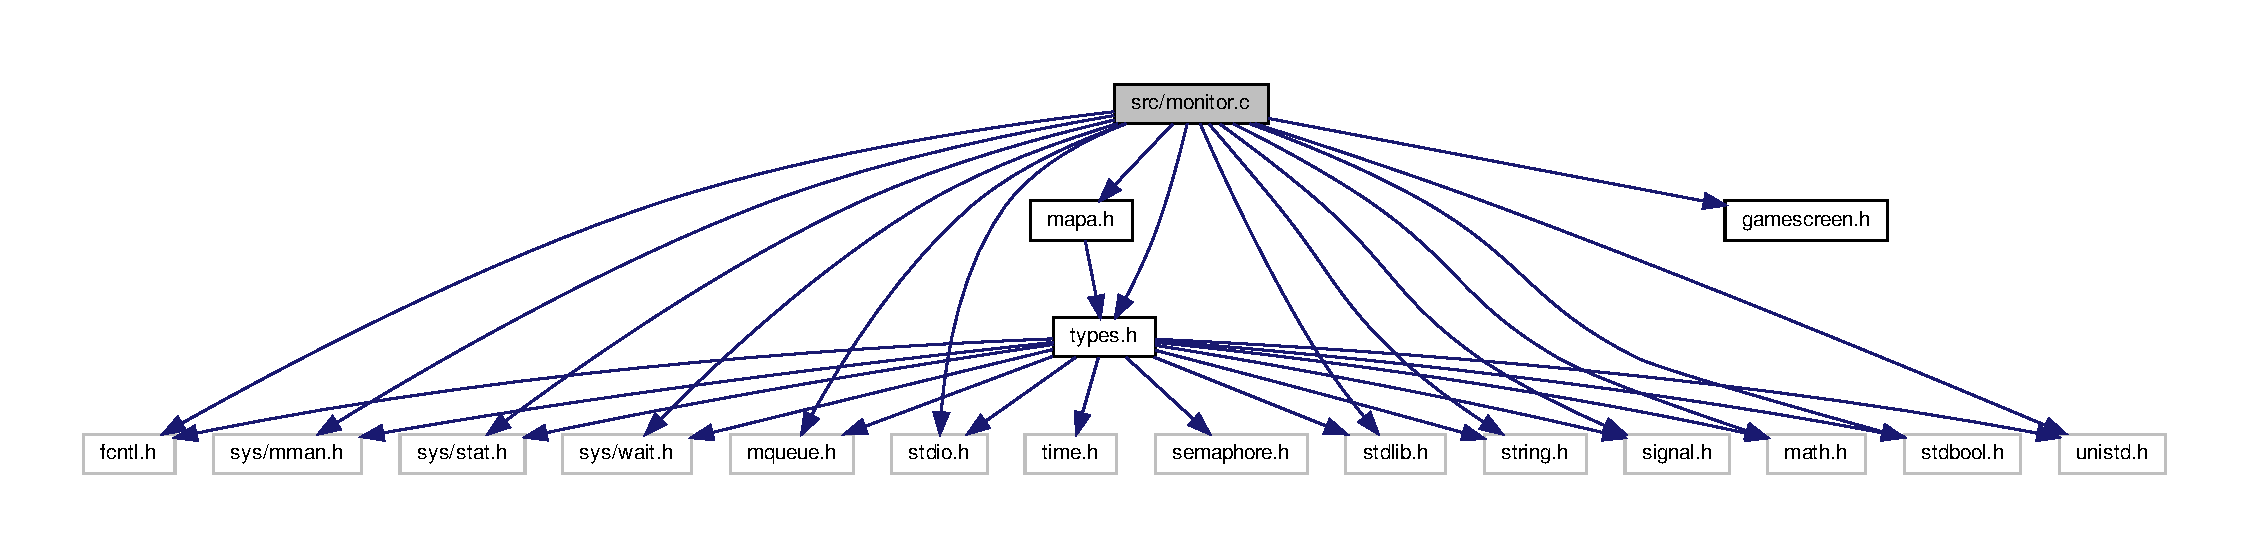
\includegraphics[width=350pt]{monitor_8c__incl}
\end{center}
\end{figure}
\subsection*{Funciones}
\begin{DoxyCompactItemize}
\item 
void \hyperlink{monitor_8c_a19b6b23fdb523f12cdc3a096dcd92d25}{mapa\+\_\+print} (\hyperlink{structtipo__mapa}{tipo\+\_\+mapa} $\ast$mapa)
\item 
void \hyperlink{monitor_8c_ac549a91c75c8860d52299ffd09451849}{monitor\+\_\+configurar\+\_\+semaforos} (sem\+\_\+t $\ast$$\ast$sem\+\_\+monitor)
\item 
void \hyperlink{monitor_8c_a2c139d68d58c9d8b1fe46230d5ac7f02}{monitor\+\_\+configurar\+\_\+memoria\+\_\+compartida} (int $\ast$shm, \hyperlink{structtipo__mapa}{tipo\+\_\+mapa} $\ast$$\ast$mapa)
\item 
void \hyperlink{monitor_8c_a1fb5c636253d81a14119899234631e04}{simulador\+\_\+configurar\+\_\+manejador} ()
\item 
void \hyperlink{monitor_8c_a9b575b72100cf87b4803476ed146be02}{manejador\+\_\+\+S\+I\+G\+I\+NT} (int pid)
\item 
int \hyperlink{monitor_8c_ae66f6b31b5ad750f1fe042a706a4e3d4}{main} ()
\end{DoxyCompactItemize}


\subsection{Descripción detallada}
Código fuente del monitor. 



\subsection{Documentación de las funciones}
\mbox{\Hypertarget{monitor_8c_ae66f6b31b5ad750f1fe042a706a4e3d4}\label{monitor_8c_ae66f6b31b5ad750f1fe042a706a4e3d4}} 
\index{monitor.\+c@{monitor.\+c}!main@{main}}
\index{main@{main}!monitor.\+c@{monitor.\+c}}
\subsubsection{\texorpdfstring{main()}{main()}}
{\footnotesize\ttfamily int main (\begin{DoxyParamCaption}{ }\end{DoxyParamCaption})}

Ejecuta el monitor \mbox{\Hypertarget{monitor_8c_a9b575b72100cf87b4803476ed146be02}\label{monitor_8c_a9b575b72100cf87b4803476ed146be02}} 
\index{monitor.\+c@{monitor.\+c}!manejador\+\_\+\+S\+I\+G\+I\+NT@{manejador\+\_\+\+S\+I\+G\+I\+NT}}
\index{manejador\+\_\+\+S\+I\+G\+I\+NT@{manejador\+\_\+\+S\+I\+G\+I\+NT}!monitor.\+c@{monitor.\+c}}
\subsubsection{\texorpdfstring{manejador\+\_\+\+S\+I\+G\+I\+N\+T()}{manejador\_SIGINT()}}
{\footnotesize\ttfamily void manejador\+\_\+\+S\+I\+G\+I\+NT (\begin{DoxyParamCaption}\item[{int}]{pid }\end{DoxyParamCaption})}

Manejador de S\+I\+G\+I\+NT. Hace \hyperlink{gamescreen_8c_af3bc8be95518f1d57d6d201a980359be}{screen\+\_\+end()} para finalizar el modo pantalla. 
\begin{DoxyParams}{Parámetros}
{\em pid} & Id del proceso\\
\hline
\end{DoxyParams}
Manejador de S\+I\+G\+I\+NT. Hace unlink de los recursos compartidos y envía S\+I\+G\+K\+I\+LL a todos los procesos de la simulación. 
\begin{DoxyParams}{Parámetros}
{\em pid} & Id del proceso \\
\hline
\end{DoxyParams}
\mbox{\Hypertarget{monitor_8c_a19b6b23fdb523f12cdc3a096dcd92d25}\label{monitor_8c_a19b6b23fdb523f12cdc3a096dcd92d25}} 
\index{monitor.\+c@{monitor.\+c}!mapa\+\_\+print@{mapa\+\_\+print}}
\index{mapa\+\_\+print@{mapa\+\_\+print}!monitor.\+c@{monitor.\+c}}
\subsubsection{\texorpdfstring{mapa\+\_\+print()}{mapa\_print()}}
{\footnotesize\ttfamily void mapa\+\_\+print (\begin{DoxyParamCaption}\item[{\hyperlink{structtipo__mapa}{tipo\+\_\+mapa} $\ast$}]{mapa }\end{DoxyParamCaption})}

Imprime el mapa 
\begin{DoxyParams}{Parámetros}
{\em mapa} & Mapa a imprimir \\
\hline
\end{DoxyParams}
\mbox{\Hypertarget{monitor_8c_a2c139d68d58c9d8b1fe46230d5ac7f02}\label{monitor_8c_a2c139d68d58c9d8b1fe46230d5ac7f02}} 
\index{monitor.\+c@{monitor.\+c}!monitor\+\_\+configurar\+\_\+memoria\+\_\+compartida@{monitor\+\_\+configurar\+\_\+memoria\+\_\+compartida}}
\index{monitor\+\_\+configurar\+\_\+memoria\+\_\+compartida@{monitor\+\_\+configurar\+\_\+memoria\+\_\+compartida}!monitor.\+c@{monitor.\+c}}
\subsubsection{\texorpdfstring{monitor\+\_\+configurar\+\_\+memoria\+\_\+compartida()}{monitor\_configurar\_memoria\_compartida()}}
{\footnotesize\ttfamily void monitor\+\_\+configurar\+\_\+memoria\+\_\+compartida (\begin{DoxyParamCaption}\item[{int $\ast$}]{shm,  }\item[{\hyperlink{structtipo__mapa}{tipo\+\_\+mapa} $\ast$$\ast$}]{mapa }\end{DoxyParamCaption})}

Configura la memoria compartida necesaria para el monitor. 
\begin{DoxyParams}{Parámetros}
{\em shm} & Referencia a la memoria compartida que se va a abrir \\
\hline
{\em mapa} & Mapa a abrir en memoria compartida \\
\hline
\end{DoxyParams}
\mbox{\Hypertarget{monitor_8c_ac549a91c75c8860d52299ffd09451849}\label{monitor_8c_ac549a91c75c8860d52299ffd09451849}} 
\index{monitor.\+c@{monitor.\+c}!monitor\+\_\+configurar\+\_\+semaforos@{monitor\+\_\+configurar\+\_\+semaforos}}
\index{monitor\+\_\+configurar\+\_\+semaforos@{monitor\+\_\+configurar\+\_\+semaforos}!monitor.\+c@{monitor.\+c}}
\subsubsection{\texorpdfstring{monitor\+\_\+configurar\+\_\+semaforos()}{monitor\_configurar\_semaforos()}}
{\footnotesize\ttfamily void monitor\+\_\+configurar\+\_\+semaforos (\begin{DoxyParamCaption}\item[{sem\+\_\+t $\ast$$\ast$}]{sem\+\_\+monitor }\end{DoxyParamCaption})}

Configura el semáforo que permite al monitor esperar hasta que comience la simulación. 
\begin{DoxyParams}{Parámetros}
{\em sem\+\_\+monitor} & Semáforo que permite al monitor esperar hasta que comience la simulación \\
\hline
\end{DoxyParams}
\mbox{\Hypertarget{monitor_8c_a1fb5c636253d81a14119899234631e04}\label{monitor_8c_a1fb5c636253d81a14119899234631e04}} 
\index{monitor.\+c@{monitor.\+c}!simulador\+\_\+configurar\+\_\+manejador@{simulador\+\_\+configurar\+\_\+manejador}}
\index{simulador\+\_\+configurar\+\_\+manejador@{simulador\+\_\+configurar\+\_\+manejador}!monitor.\+c@{monitor.\+c}}
\subsubsection{\texorpdfstring{simulador\+\_\+configurar\+\_\+manejador()}{simulador\_configurar\_manejador()}}
{\footnotesize\ttfamily void simulador\+\_\+configurar\+\_\+manejador (\begin{DoxyParamCaption}{ }\end{DoxyParamCaption})}

Crea el manejador de S\+I\+G\+I\+NT, en caso de que se desee interrumpir la ejecución a mitad del proceso. 
\hypertarget{nave_8c}{}\section{Referencia del Archivo src/nave.c}
\label{nave_8c}\index{src/nave.\+c@{src/nave.\+c}}


Codigo fuente de nave.  


{\ttfamily \#include \char`\"{}nave.\+h\char`\"{}}\newline
Dependencia gráfica adjunta para nave.\+c\+:
\nopagebreak
\begin{figure}[H]
\begin{center}
\leavevmode
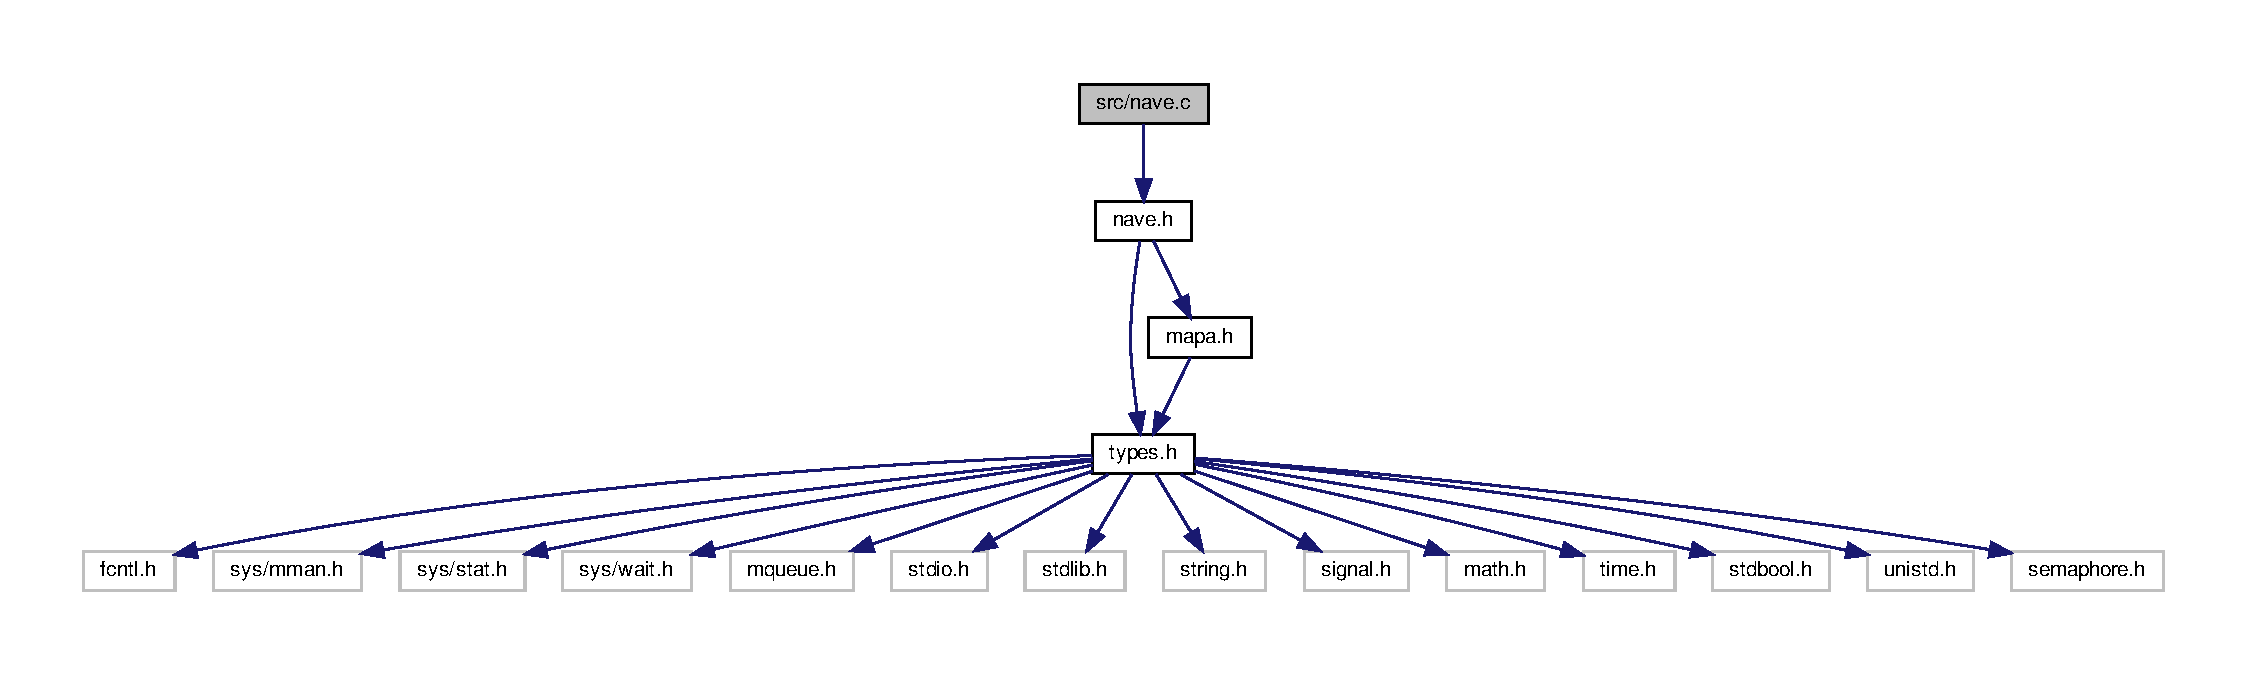
\includegraphics[width=350pt]{nave_8c__incl}
\end{center}
\end{figure}
\subsection*{Funciones}
\begin{DoxyCompactItemize}
\item 
void \hyperlink{nave_8c_a1add2308319c21965be67ae8d3099296}{nave\+\_\+configurar\+\_\+cola} (int n\+\_\+equipo, int n\+\_\+nave, mqd\+\_\+t $\ast$cola)
\item 
void \hyperlink{nave_8c_a3d3f3f9b58aa6d6db95e19023d33f163}{nave} (\hyperlink{structtipo__mapa}{tipo\+\_\+mapa} $\ast$mapa, int n\+\_\+equipo, int n\+\_\+nave, int fd\+\_\+jefe\mbox{[}2\mbox{]})
\end{DoxyCompactItemize}


\subsection{Descripción detallada}
Codigo fuente de nave. 



\subsection{Documentación de las funciones}
\mbox{\Hypertarget{nave_8c_a3d3f3f9b58aa6d6db95e19023d33f163}\label{nave_8c_a3d3f3f9b58aa6d6db95e19023d33f163}} 
\index{nave.\+c@{nave.\+c}!nave@{nave}}
\index{nave@{nave}!nave.\+c@{nave.\+c}}
\subsubsection{\texorpdfstring{nave()}{nave()}}
{\footnotesize\ttfamily void nave (\begin{DoxyParamCaption}\item[{\hyperlink{structtipo__mapa}{tipo\+\_\+mapa} $\ast$}]{mapa,  }\item[{int}]{n\+\_\+equipo,  }\item[{int}]{n\+\_\+nave,  }\item[{int}]{fd\+\_\+jefe\mbox{[}2\mbox{]} }\end{DoxyParamCaption})}

Emula el comportamiento de una nave, \char`\"{}obedeciendo\char`\"{} las órdenes de su jefe e informando de sus acciones al simulador. 
\begin{DoxyParams}{Parámetros}
{\em mapa} & Mapa sobre el que se situa la nave \\
\hline
{\em n\+\_\+equipo} & Número de equipo de la nave \\
\hline
{\em n\+\_\+nave} & Número de la nave \\
\hline
{\em fd\+\_\+jefe} & Pipe que conecta la nave con su jefe \\
\hline
\end{DoxyParams}
\begin{DoxySeeAlso}{Ver también}
\hyperlink{jefe_8c_acc2874834095a0921d3b644130bfb4c6}{jefe()} 

\hyperlink{simulador_8c_a7ca1584ef7c92847d2a610dffac0ccba}{simulador()} 
\end{DoxySeeAlso}
\mbox{\Hypertarget{nave_8c_a1add2308319c21965be67ae8d3099296}\label{nave_8c_a1add2308319c21965be67ae8d3099296}} 
\index{nave.\+c@{nave.\+c}!nave\+\_\+configurar\+\_\+cola@{nave\+\_\+configurar\+\_\+cola}}
\index{nave\+\_\+configurar\+\_\+cola@{nave\+\_\+configurar\+\_\+cola}!nave.\+c@{nave.\+c}}
\subsubsection{\texorpdfstring{nave\+\_\+configurar\+\_\+cola()}{nave\_configurar\_cola()}}
{\footnotesize\ttfamily void nave\+\_\+configurar\+\_\+cola (\begin{DoxyParamCaption}\item[{int}]{n\+\_\+equipo,  }\item[{int}]{n\+\_\+nave,  }\item[{mqd\+\_\+t $\ast$}]{cola }\end{DoxyParamCaption})}

Configura la cola de mensajes que comunica a la nave con el simulador 
\begin{DoxyParams}{Parámetros}
{\em n\+\_\+equipo} & Número de equipo de la nave \\
\hline
{\em n\+\_\+equipo} & Número de la nave \\
\hline
{\em cola} & Cola de mensajes a configurar \\
\hline
\end{DoxyParams}

\hypertarget{nave_8h}{}\section{Referencia del Archivo src/nave.h}
\label{nave_8h}\index{src/nave.\+h@{src/nave.\+h}}


Recoge la funcionalidad de una nave.  


{\ttfamily \#include \char`\"{}types.\+h\char`\"{}}\newline
{\ttfamily \#include \char`\"{}mapa.\+h\char`\"{}}\newline
Dependencia gráfica adjunta para nave.\+h\+:
\nopagebreak
\begin{figure}[H]
\begin{center}
\leavevmode
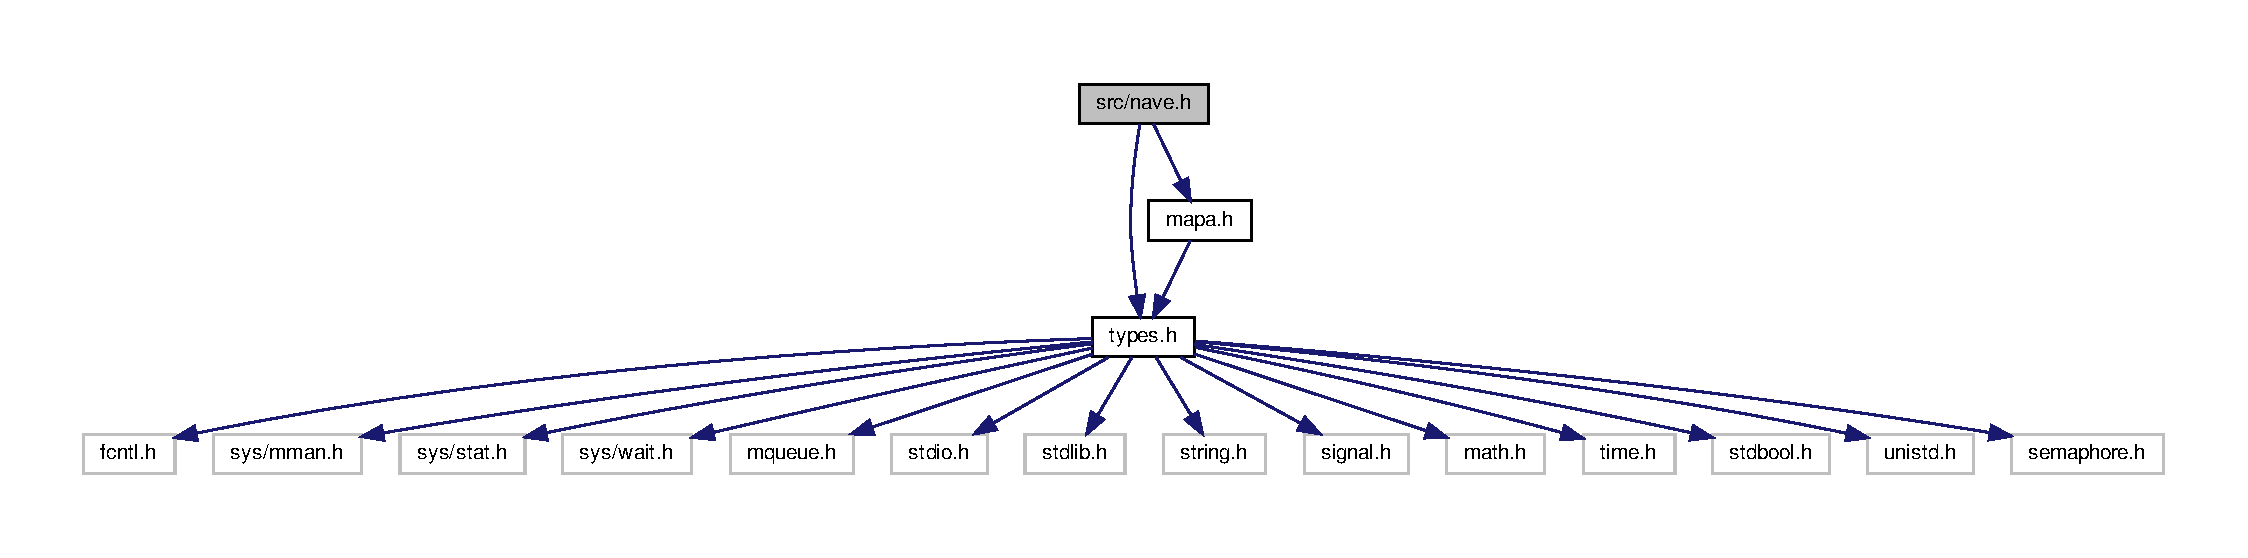
\includegraphics[width=350pt]{nave_8h__incl}
\end{center}
\end{figure}
Gráfico de los archivos que directa o indirectamente incluyen a este archivo\+:
\nopagebreak
\begin{figure}[H]
\begin{center}
\leavevmode
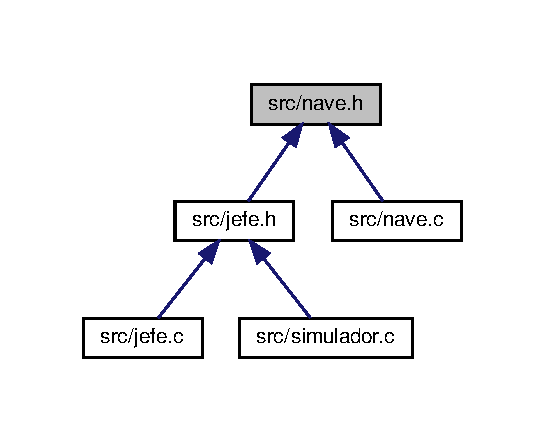
\includegraphics[width=262pt]{nave_8h__dep__incl}
\end{center}
\end{figure}
\subsection*{Funciones}
\begin{DoxyCompactItemize}
\item 
void \hyperlink{nave_8h_a3d3f3f9b58aa6d6db95e19023d33f163}{nave} (\hyperlink{structtipo__mapa}{tipo\+\_\+mapa} $\ast$mapa, int n\+\_\+equipo, int n\+\_\+nave, int fd\+\_\+jefe\mbox{[}2\mbox{]})
\end{DoxyCompactItemize}


\subsection{Descripción detallada}
Recoge la funcionalidad de una nave. 



\subsection{Documentación de las funciones}
\mbox{\Hypertarget{nave_8h_a3d3f3f9b58aa6d6db95e19023d33f163}\label{nave_8h_a3d3f3f9b58aa6d6db95e19023d33f163}} 
\index{nave.\+h@{nave.\+h}!nave@{nave}}
\index{nave@{nave}!nave.\+h@{nave.\+h}}
\subsubsection{\texorpdfstring{nave()}{nave()}}
{\footnotesize\ttfamily void nave (\begin{DoxyParamCaption}\item[{\hyperlink{structtipo__mapa}{tipo\+\_\+mapa} $\ast$}]{mapa,  }\item[{int}]{n\+\_\+equipo,  }\item[{int}]{n\+\_\+nave,  }\item[{int}]{fd\+\_\+jefe\mbox{[}2\mbox{]} }\end{DoxyParamCaption})}

Emula el comportamiento de una nave, \char`\"{}obedeciendo\char`\"{} las órdenes de su jefe e informando de sus acciones al simulador. 
\begin{DoxyParams}{Parámetros}
{\em mapa} & Mapa sobre el que se situa la nave \\
\hline
{\em n\+\_\+equipo} & Número de equipo de la nave \\
\hline
{\em n\+\_\+nave} & Número de la nave \\
\hline
{\em fd\+\_\+jefe} & Pipe que conecta la nave con su jefe \\
\hline
\end{DoxyParams}
\begin{DoxySeeAlso}{Ver también}
\hyperlink{jefe_8c_acc2874834095a0921d3b644130bfb4c6}{jefe()} 

\hyperlink{simulador_8c_a7ca1584ef7c92847d2a610dffac0ccba}{simulador()} 
\end{DoxySeeAlso}

\hypertarget{simulador_8c}{}\section{Referencia del Archivo src/simulador.c}
\label{simulador_8c}\index{src/simulador.\+c@{src/simulador.\+c}}


Código fuente del simulador.  


{\ttfamily \#include \char`\"{}jefe.\+h\char`\"{}}\newline
{\ttfamily \#include \char`\"{}mapa.\+h\char`\"{}}\newline
{\ttfamily \#include \char`\"{}types.\+h\char`\"{}}\newline
Dependencia gráfica adjunta para simulador.\+c\+:
\nopagebreak
\begin{figure}[H]
\begin{center}
\leavevmode
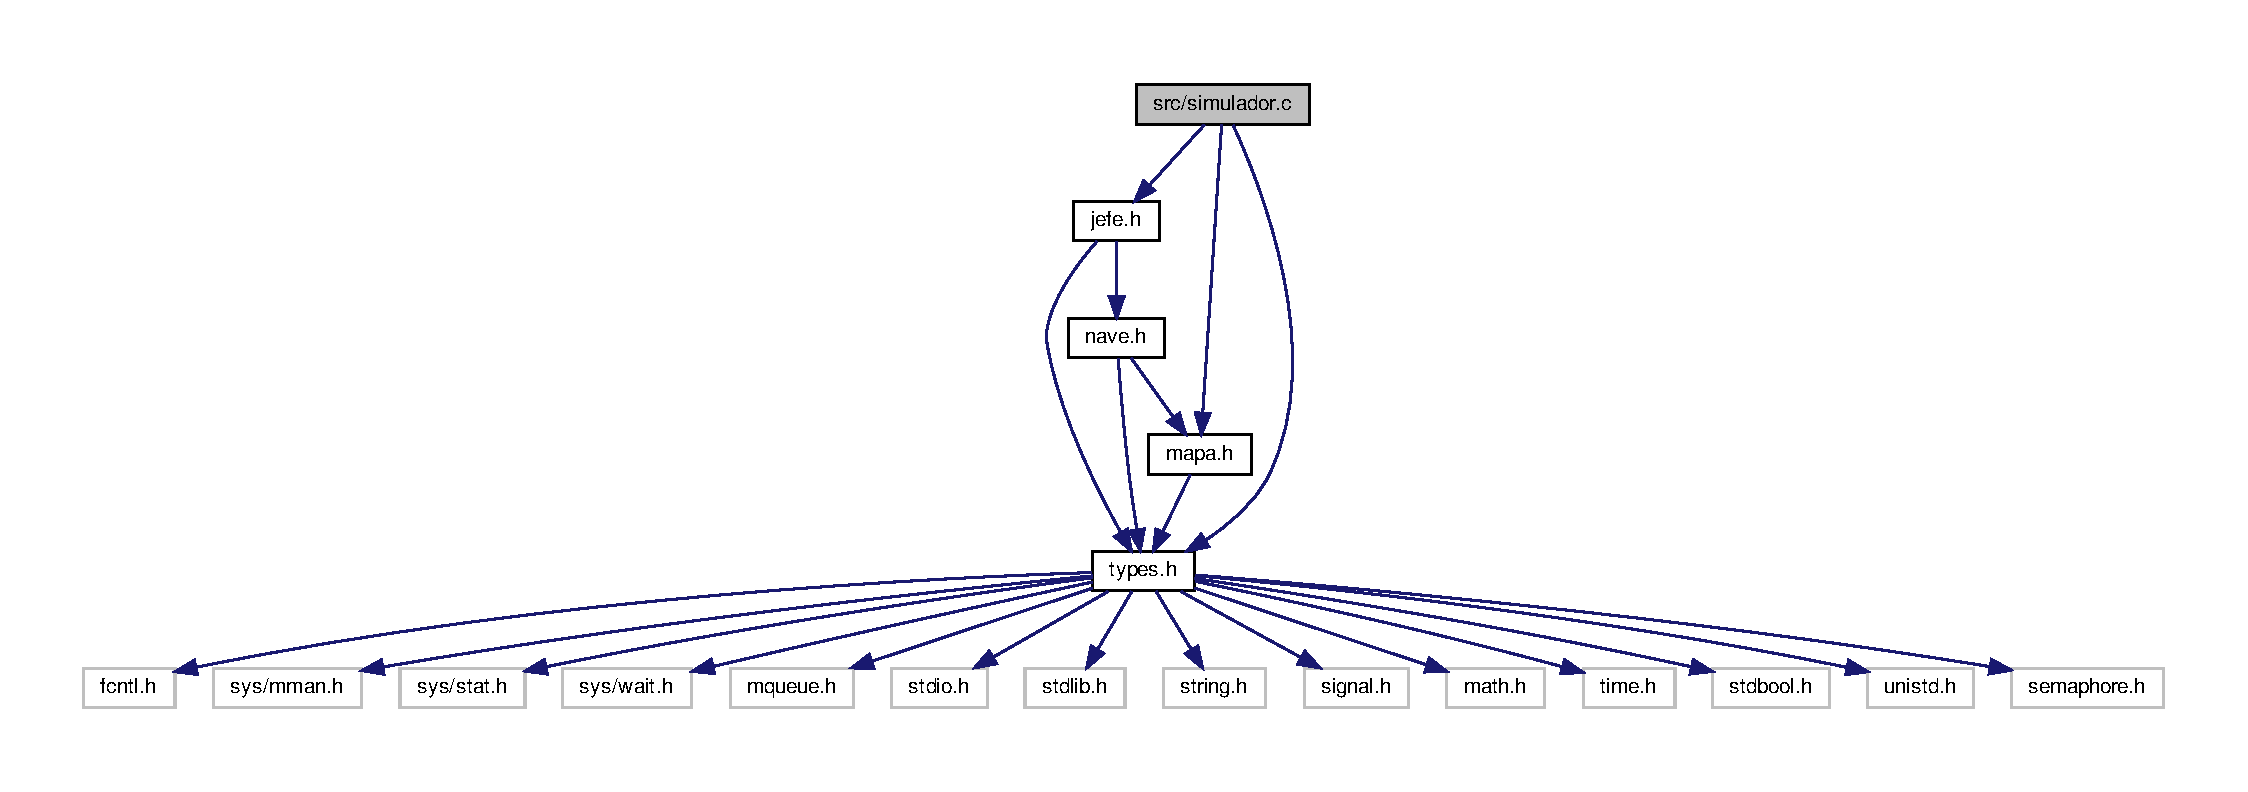
\includegraphics[width=350pt]{simulador_8c__incl}
\end{center}
\end{figure}
\subsection*{Funciones}
\begin{DoxyCompactItemize}
\item 
void \hyperlink{simulador_8c_a7ca1584ef7c92847d2a610dffac0ccba}{simulador} ()
\item 
void \hyperlink{simulador_8c_a844708a2e47c074af2c3df7bbc08debe}{simulador\+\_\+crear\+\_\+jefes} (\hyperlink{structtipo__mapa}{tipo\+\_\+mapa} $\ast$mapa, int fd\+\_\+sim\mbox{[}\hyperlink{types_8h_ab306668933fb4316ac0f5ef291d13dff}{N\+\_\+\+E\+Q\+U\+I\+P\+OS}\mbox{]}\mbox{[}2\mbox{]}, sem\+\_\+t $\ast$sem\+\_\+equipos\+\_\+listos)
\item 
void \hyperlink{simulador_8c_aafad343d1f6fcf94e098090354257fec}{simulador\+\_\+configurar\+\_\+semaforos} (sem\+\_\+t $\ast$$\ast$sem\+\_\+monitor, sem\+\_\+t $\ast$$\ast$sem\+\_\+equipos\+\_\+listos)
\item 
void \hyperlink{simulador_8c_ab7458076c9646b481352dbcaa4962ff4}{simulador\+\_\+configurar\+\_\+manejadores} ()
\item 
void \hyperlink{simulador_8c_ab6ce2c925b1ddbd366f414e246565bfb}{simulador\+\_\+configurar\+\_\+cola} (mqd\+\_\+t $\ast$cola)
\item 
void \hyperlink{simulador_8c_a28bc47609f58946ba64fb3dd386819c0}{simulador\+\_\+configurar\+\_\+memoria\+\_\+compartida} (int $\ast$shm, \hyperlink{structtipo__mapa}{tipo\+\_\+mapa} $\ast$$\ast$mapa)
\item 
void \hyperlink{simulador_8c_a7a757062b703107b35d26563c82d07d7}{simulador\+\_\+configurar\+\_\+mapa} (\hyperlink{structtipo__mapa}{tipo\+\_\+mapa} $\ast$mapa)
\item 
void \hyperlink{simulador_8c_ac3ea499f27bd220f1d39122cce587119}{simulador\+\_\+configurar\+\_\+naves} (\hyperlink{structtipo__mapa}{tipo\+\_\+mapa} $\ast$mapa)
\item 
void \hyperlink{simulador_8c_a9b575b72100cf87b4803476ed146be02}{manejador\+\_\+\+S\+I\+G\+I\+NT} (int pid)
\item 
void \hyperlink{simulador_8c_a1f0c3c2b53531f97806cd6db2f5c68e0}{manejador\+\_\+\+S\+I\+G\+A\+L\+RM} (int pid)
\item 
void \hyperlink{simulador_8c_a69385757034f67a3cd63887bdc544b69}{manejador\+\_\+\+S\+I\+G\+T\+E\+RM} (int pid)
\item 
int \hyperlink{simulador_8c_ae66f6b31b5ad750f1fe042a706a4e3d4}{main} ()
\end{DoxyCompactItemize}
\subsection*{Variables}
\begin{DoxyCompactItemize}
\item 
\mbox{\Hypertarget{simulador_8c_a350a4b7e3f7ddadd409eb761bbfb28cb}\label{simulador_8c_a350a4b7e3f7ddadd409eb761bbfb28cb}} 
sem\+\_\+t $\ast$ {\bfseries sem\+\_\+alarma} = N\+U\+LL
\end{DoxyCompactItemize}


\subsection{Descripción detallada}
Código fuente del simulador. 



\subsection{Documentación de las funciones}
\mbox{\Hypertarget{simulador_8c_ae66f6b31b5ad750f1fe042a706a4e3d4}\label{simulador_8c_ae66f6b31b5ad750f1fe042a706a4e3d4}} 
\index{simulador.\+c@{simulador.\+c}!main@{main}}
\index{main@{main}!simulador.\+c@{simulador.\+c}}
\subsubsection{\texorpdfstring{main()}{main()}}
{\footnotesize\ttfamily int main (\begin{DoxyParamCaption}{ }\end{DoxyParamCaption})}

Ejecuta el simulador \mbox{\Hypertarget{simulador_8c_a1f0c3c2b53531f97806cd6db2f5c68e0}\label{simulador_8c_a1f0c3c2b53531f97806cd6db2f5c68e0}} 
\index{simulador.\+c@{simulador.\+c}!manejador\+\_\+\+S\+I\+G\+A\+L\+RM@{manejador\+\_\+\+S\+I\+G\+A\+L\+RM}}
\index{manejador\+\_\+\+S\+I\+G\+A\+L\+RM@{manejador\+\_\+\+S\+I\+G\+A\+L\+RM}!simulador.\+c@{simulador.\+c}}
\subsubsection{\texorpdfstring{manejador\+\_\+\+S\+I\+G\+A\+L\+R\+M()}{manejador\_SIGALRM()}}
{\footnotesize\ttfamily void manejador\+\_\+\+S\+I\+G\+A\+L\+RM (\begin{DoxyParamCaption}\item[{int}]{pid }\end{DoxyParamCaption})}

Manejador de S\+I\+G\+A\+L\+A\+RM. Sube el semáforo que permite el fin del turno. \mbox{\Hypertarget{simulador_8c_a9b575b72100cf87b4803476ed146be02}\label{simulador_8c_a9b575b72100cf87b4803476ed146be02}} 
\index{simulador.\+c@{simulador.\+c}!manejador\+\_\+\+S\+I\+G\+I\+NT@{manejador\+\_\+\+S\+I\+G\+I\+NT}}
\index{manejador\+\_\+\+S\+I\+G\+I\+NT@{manejador\+\_\+\+S\+I\+G\+I\+NT}!simulador.\+c@{simulador.\+c}}
\subsubsection{\texorpdfstring{manejador\+\_\+\+S\+I\+G\+I\+N\+T()}{manejador\_SIGINT()}}
{\footnotesize\ttfamily void manejador\+\_\+\+S\+I\+G\+I\+NT (\begin{DoxyParamCaption}\item[{int}]{pid }\end{DoxyParamCaption})}

Manejador de S\+I\+G\+I\+NT. Hace unlink de los recursos compartidos y envía S\+I\+G\+K\+I\+LL a todos los procesos de la simulación. 
\begin{DoxyParams}{Parámetros}
{\em pid} & Id del proceso \\
\hline
\end{DoxyParams}
\mbox{\Hypertarget{simulador_8c_a69385757034f67a3cd63887bdc544b69}\label{simulador_8c_a69385757034f67a3cd63887bdc544b69}} 
\index{simulador.\+c@{simulador.\+c}!manejador\+\_\+\+S\+I\+G\+T\+E\+RM@{manejador\+\_\+\+S\+I\+G\+T\+E\+RM}}
\index{manejador\+\_\+\+S\+I\+G\+T\+E\+RM@{manejador\+\_\+\+S\+I\+G\+T\+E\+RM}!simulador.\+c@{simulador.\+c}}
\subsubsection{\texorpdfstring{manejador\+\_\+\+S\+I\+G\+T\+E\+R\+M()}{manejador\_SIGTERM()}}
{\footnotesize\ttfamily void manejador\+\_\+\+S\+I\+G\+T\+E\+RM (\begin{DoxyParamCaption}\item[{int}]{pid }\end{DoxyParamCaption})}

Manejador de S\+I\+G\+T\+E\+RM. Finaliza la ejecución. \mbox{\Hypertarget{simulador_8c_a7ca1584ef7c92847d2a610dffac0ccba}\label{simulador_8c_a7ca1584ef7c92847d2a610dffac0ccba}} 
\index{simulador.\+c@{simulador.\+c}!simulador@{simulador}}
\index{simulador@{simulador}!simulador.\+c@{simulador.\+c}}
\subsubsection{\texorpdfstring{simulador()}{simulador()}}
{\footnotesize\ttfamily void simulador (\begin{DoxyParamCaption}{ }\end{DoxyParamCaption})}

Inicializa los recursos compartidos, crea los jefes y ejecuta el bucle principal del simulador hasta termina la batalla. Al finalizar libera los recursos compartidos. \mbox{\Hypertarget{simulador_8c_ab6ce2c925b1ddbd366f414e246565bfb}\label{simulador_8c_ab6ce2c925b1ddbd366f414e246565bfb}} 
\index{simulador.\+c@{simulador.\+c}!simulador\+\_\+configurar\+\_\+cola@{simulador\+\_\+configurar\+\_\+cola}}
\index{simulador\+\_\+configurar\+\_\+cola@{simulador\+\_\+configurar\+\_\+cola}!simulador.\+c@{simulador.\+c}}
\subsubsection{\texorpdfstring{simulador\+\_\+configurar\+\_\+cola()}{simulador\_configurar\_cola()}}
{\footnotesize\ttfamily void simulador\+\_\+configurar\+\_\+cola (\begin{DoxyParamCaption}\item[{mqd\+\_\+t $\ast$}]{cola }\end{DoxyParamCaption})}

Abre o crea la cola de mensajes utilizada para que las naves comuniquen sus acciones al simulador. 
\begin{DoxyParams}{Parámetros}
{\em cola} & Cola de mensajes \\
\hline
\end{DoxyParams}
\mbox{\Hypertarget{simulador_8c_ab7458076c9646b481352dbcaa4962ff4}\label{simulador_8c_ab7458076c9646b481352dbcaa4962ff4}} 
\index{simulador.\+c@{simulador.\+c}!simulador\+\_\+configurar\+\_\+manejadores@{simulador\+\_\+configurar\+\_\+manejadores}}
\index{simulador\+\_\+configurar\+\_\+manejadores@{simulador\+\_\+configurar\+\_\+manejadores}!simulador.\+c@{simulador.\+c}}
\subsubsection{\texorpdfstring{simulador\+\_\+configurar\+\_\+manejadores()}{simulador\_configurar\_manejadores()}}
{\footnotesize\ttfamily void simulador\+\_\+configurar\+\_\+manejadores (\begin{DoxyParamCaption}{ }\end{DoxyParamCaption})}

Crea los manejadores de las señales utilizadas. S\+I\+G\+I\+NT en caso de que se desee interrumpir la ejecución a mitad del proceso, S\+I\+G\+A\+L\+RM para la duración de los turnos y S\+I\+G\+T\+E\+RM para que las naves finalicen cuando los jefes se lo ordenen. \mbox{\Hypertarget{simulador_8c_a7a757062b703107b35d26563c82d07d7}\label{simulador_8c_a7a757062b703107b35d26563c82d07d7}} 
\index{simulador.\+c@{simulador.\+c}!simulador\+\_\+configurar\+\_\+mapa@{simulador\+\_\+configurar\+\_\+mapa}}
\index{simulador\+\_\+configurar\+\_\+mapa@{simulador\+\_\+configurar\+\_\+mapa}!simulador.\+c@{simulador.\+c}}
\subsubsection{\texorpdfstring{simulador\+\_\+configurar\+\_\+mapa()}{simulador\_configurar\_mapa()}}
{\footnotesize\ttfamily void simulador\+\_\+configurar\+\_\+mapa (\begin{DoxyParamCaption}\item[{\hyperlink{structtipo__mapa}{tipo\+\_\+mapa} $\ast$}]{mapa }\end{DoxyParamCaption})}

Inicializa todas las casillas del mapa de la simulación 
\begin{DoxyParams}{Parámetros}
{\em mapa} & Mapa de la simulación. \\
\hline
\end{DoxyParams}
\mbox{\Hypertarget{simulador_8c_a28bc47609f58946ba64fb3dd386819c0}\label{simulador_8c_a28bc47609f58946ba64fb3dd386819c0}} 
\index{simulador.\+c@{simulador.\+c}!simulador\+\_\+configurar\+\_\+memoria\+\_\+compartida@{simulador\+\_\+configurar\+\_\+memoria\+\_\+compartida}}
\index{simulador\+\_\+configurar\+\_\+memoria\+\_\+compartida@{simulador\+\_\+configurar\+\_\+memoria\+\_\+compartida}!simulador.\+c@{simulador.\+c}}
\subsubsection{\texorpdfstring{simulador\+\_\+configurar\+\_\+memoria\+\_\+compartida()}{simulador\_configurar\_memoria\_compartida()}}
{\footnotesize\ttfamily void simulador\+\_\+configurar\+\_\+memoria\+\_\+compartida (\begin{DoxyParamCaption}\item[{int $\ast$}]{shm,  }\item[{\hyperlink{structtipo__mapa}{tipo\+\_\+mapa} $\ast$$\ast$}]{mapa }\end{DoxyParamCaption})}

Crea la memoria compartida en la que se almacena el mapa de la simulación. 
\begin{DoxyParams}{Parámetros}
{\em shm} & Memoria compartida que se debe crear \\
\hline
{\em mapa} & Mapa almacenado en la memoria compartida \\
\hline
\end{DoxyParams}
\mbox{\Hypertarget{simulador_8c_ac3ea499f27bd220f1d39122cce587119}\label{simulador_8c_ac3ea499f27bd220f1d39122cce587119}} 
\index{simulador.\+c@{simulador.\+c}!simulador\+\_\+configurar\+\_\+naves@{simulador\+\_\+configurar\+\_\+naves}}
\index{simulador\+\_\+configurar\+\_\+naves@{simulador\+\_\+configurar\+\_\+naves}!simulador.\+c@{simulador.\+c}}
\subsubsection{\texorpdfstring{simulador\+\_\+configurar\+\_\+naves()}{simulador\_configurar\_naves()}}
{\footnotesize\ttfamily void simulador\+\_\+configurar\+\_\+naves (\begin{DoxyParamCaption}\item[{\hyperlink{structtipo__mapa}{tipo\+\_\+mapa} $\ast$}]{mapa }\end{DoxyParamCaption})}

Configura y añade al mapa las naves de los diferentes equipos, que aparecen en las cuatro esquinas del mapa. 
\begin{DoxyParams}{Parámetros}
{\em mapa} & Mapa de la simulación. \\
\hline
\end{DoxyParams}
\mbox{\Hypertarget{simulador_8c_aafad343d1f6fcf94e098090354257fec}\label{simulador_8c_aafad343d1f6fcf94e098090354257fec}} 
\index{simulador.\+c@{simulador.\+c}!simulador\+\_\+configurar\+\_\+semaforos@{simulador\+\_\+configurar\+\_\+semaforos}}
\index{simulador\+\_\+configurar\+\_\+semaforos@{simulador\+\_\+configurar\+\_\+semaforos}!simulador.\+c@{simulador.\+c}}
\subsubsection{\texorpdfstring{simulador\+\_\+configurar\+\_\+semaforos()}{simulador\_configurar\_semaforos()}}
{\footnotesize\ttfamily void simulador\+\_\+configurar\+\_\+semaforos (\begin{DoxyParamCaption}\item[{sem\+\_\+t $\ast$$\ast$}]{sem\+\_\+monitor,  }\item[{sem\+\_\+t $\ast$$\ast$}]{sem\+\_\+equipos\+\_\+listos }\end{DoxyParamCaption})}

Crea los semáforos necesarias para comunicarse con el monitor y los jefes. 
\begin{DoxyParams}{Parámetros}
{\em sem\+\_\+monitor} & Semáforo para comunicarse con el monitor \\
\hline
{\em sem\+\_\+equipos\+\_\+listos} & Semáforo para comunicarse con los jefes \\
\hline
\end{DoxyParams}
\mbox{\Hypertarget{simulador_8c_a844708a2e47c074af2c3df7bbc08debe}\label{simulador_8c_a844708a2e47c074af2c3df7bbc08debe}} 
\index{simulador.\+c@{simulador.\+c}!simulador\+\_\+crear\+\_\+jefes@{simulador\+\_\+crear\+\_\+jefes}}
\index{simulador\+\_\+crear\+\_\+jefes@{simulador\+\_\+crear\+\_\+jefes}!simulador.\+c@{simulador.\+c}}
\subsubsection{\texorpdfstring{simulador\+\_\+crear\+\_\+jefes()}{simulador\_crear\_jefes()}}
{\footnotesize\ttfamily void simulador\+\_\+crear\+\_\+jefes (\begin{DoxyParamCaption}\item[{\hyperlink{structtipo__mapa}{tipo\+\_\+mapa} $\ast$}]{mapa,  }\item[{int}]{fd\+\_\+sim\mbox{[}\+N\+\_\+\+E\+Q\+U\+I\+P\+O\+S\mbox{]}\mbox{[}2\mbox{]},  }\item[{sem\+\_\+t $\ast$}]{sem\+\_\+equipos\+\_\+listos }\end{DoxyParamCaption})}

Crea procesos para cada jefe, junto a tuberías para mantener la comunicación 
\begin{DoxyParams}{Parámetros}
{\em mapa} & Mapa de la simulación \\
\hline
{\em fd\+\_\+sim} & Tuberías que se deben crear \\
\hline
{\em sem\+\_\+equipos\+\_\+listos} & Semáforo que se pasará a los jefes \\
\hline
\end{DoxyParams}

\hypertarget{types_8h}{}\section{Referencia del Archivo src/types.h}
\label{types_8h}\index{src/types.\+h@{src/types.\+h}}


Define los tipos y constantes de datos.  


{\ttfamily \#include $<$fcntl.\+h$>$}\newline
{\ttfamily \#include $<$sys/mman.\+h$>$}\newline
{\ttfamily \#include $<$sys/stat.\+h$>$}\newline
{\ttfamily \#include $<$sys/wait.\+h$>$}\newline
{\ttfamily \#include $<$mqueue.\+h$>$}\newline
{\ttfamily \#include $<$stdio.\+h$>$}\newline
{\ttfamily \#include $<$stdlib.\+h$>$}\newline
{\ttfamily \#include $<$string.\+h$>$}\newline
{\ttfamily \#include $<$signal.\+h$>$}\newline
{\ttfamily \#include $<$math.\+h$>$}\newline
{\ttfamily \#include $<$time.\+h$>$}\newline
{\ttfamily \#include $<$stdbool.\+h$>$}\newline
{\ttfamily \#include $<$unistd.\+h$>$}\newline
{\ttfamily \#include $<$semaphore.\+h$>$}\newline
Dependencia gráfica adjunta para types.\+h\+:
\nopagebreak
\begin{figure}[H]
\begin{center}
\leavevmode
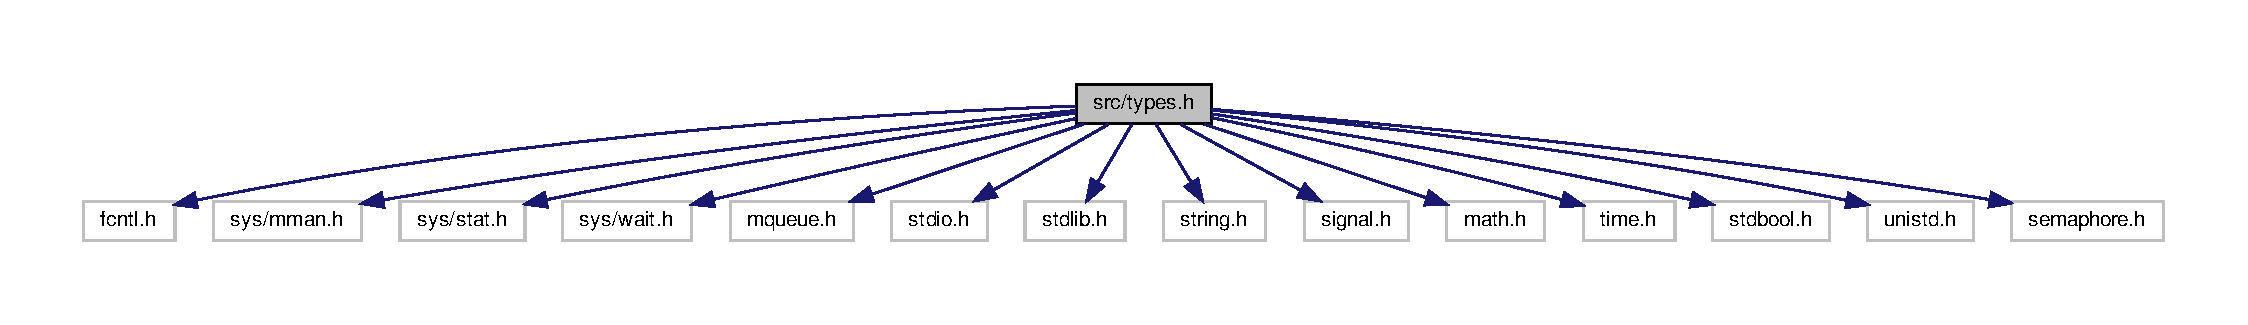
\includegraphics[width=350pt]{types_8h__incl}
\end{center}
\end{figure}
Gráfico de los archivos que directa o indirectamente incluyen a este archivo\+:
\nopagebreak
\begin{figure}[H]
\begin{center}
\leavevmode
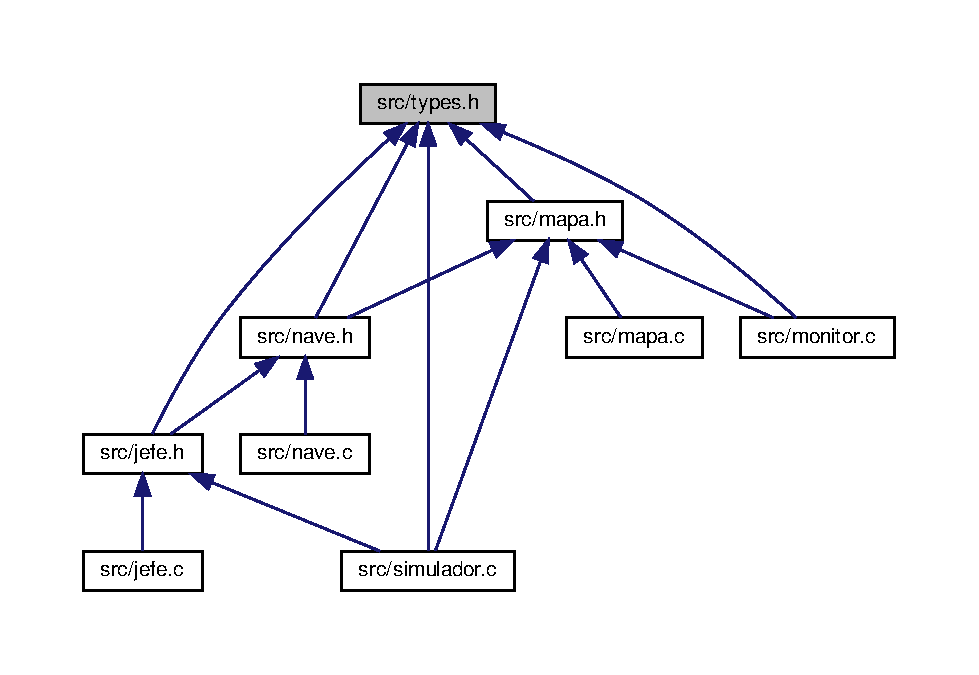
\includegraphics[width=350pt]{types_8h__dep__incl}
\end{center}
\end{figure}
\subsection*{Clases}
\begin{DoxyCompactItemize}
\item 
struct \hyperlink{structMensaje}{Mensaje}
\item 
struct \hyperlink{structtipo__nave}{tipo\+\_\+nave}
\item 
struct \hyperlink{structtipo__casilla}{tipo\+\_\+casilla}
\item 
struct \hyperlink{structtipo__mapa}{tipo\+\_\+mapa}
\end{DoxyCompactItemize}
\subsection*{defines}
\begin{DoxyCompactItemize}
\item 
\mbox{\Hypertarget{types_8h_ab306668933fb4316ac0f5ef291d13dff}\label{types_8h_ab306668933fb4316ac0f5ef291d13dff}} 
\#define \hyperlink{types_8h_ab306668933fb4316ac0f5ef291d13dff}{N\+\_\+\+E\+Q\+U\+I\+P\+OS}~4
\begin{DoxyCompactList}\small\item\em Número de equipos. \end{DoxyCompactList}\item 
\mbox{\Hypertarget{types_8h_aa1f2aba814c6d46772f9694849eeaa7a}\label{types_8h_aa1f2aba814c6d46772f9694849eeaa7a}} 
\#define \hyperlink{types_8h_aa1f2aba814c6d46772f9694849eeaa7a}{N\+\_\+\+N\+A\+V\+ES}~3
\begin{DoxyCompactList}\small\item\em Número de naves por equipo. \end{DoxyCompactList}\item 
\mbox{\Hypertarget{types_8h_a6b20d41d6252e9871430c242cb1a56e7}\label{types_8h_a6b20d41d6252e9871430c242cb1a56e7}} 
\#define \hyperlink{types_8h_a6b20d41d6252e9871430c242cb1a56e7}{B\+U\+F\+F\+E\+R\+\_\+\+S\+I\+ZE}~80
\begin{DoxyCompactList}\small\item\em Tamaño del buffer que se usa para leer de los pipes. \end{DoxyCompactList}\item 
\mbox{\Hypertarget{types_8h_ae0b4816fb45161ef9da5e6d6134ee28a}\label{types_8h_ae0b4816fb45161ef9da5e6d6134ee28a}} 
\#define \hyperlink{types_8h_ae0b4816fb45161ef9da5e6d6134ee28a}{T\+AM}~256
\begin{DoxyCompactList}\small\item\em Tamaño máximo de los mensajes. \end{DoxyCompactList}\item 
\mbox{\Hypertarget{types_8h_aa24597a54a085c6c2c33b64138f09eff}\label{types_8h_aa24597a54a085c6c2c33b64138f09eff}} 
\#define \hyperlink{types_8h_aa24597a54a085c6c2c33b64138f09eff}{M\+A\+X\+\_\+\+M\+SG}~10
\begin{DoxyCompactList}\small\item\em Número máximo de mensajes en la cola. \end{DoxyCompactList}\item 
\mbox{\Hypertarget{types_8h_a8e4f437d2c4b0bdd426658073d9427a7}\label{types_8h_a8e4f437d2c4b0bdd426658073d9427a7}} 
\#define \hyperlink{types_8h_a8e4f437d2c4b0bdd426658073d9427a7}{T\+U\+R\+NO}~\char`\"{}turno\char`\"{}
\begin{DoxyCompactList}\small\item\em \hyperlink{structMensaje}{Mensaje} que envía el simulador a los jefes para indicar que es un turno nuevo. \end{DoxyCompactList}\item 
\mbox{\Hypertarget{types_8h_a1ce3da0d4a8e4638874faeae3b66fbcc}\label{types_8h_a1ce3da0d4a8e4638874faeae3b66fbcc}} 
\#define \hyperlink{types_8h_a1ce3da0d4a8e4638874faeae3b66fbcc}{F\+IN}~\char`\"{}fin\char`\"{}
\begin{DoxyCompactList}\small\item\em \hyperlink{structMensaje}{Mensaje} que envía el simulador a los jefes para que estos finalicen. \end{DoxyCompactList}\item 
\mbox{\Hypertarget{types_8h_a3905426db8ac81dee33ae9b1bfe87686}\label{types_8h_a3905426db8ac81dee33ae9b1bfe87686}} 
\#define \hyperlink{types_8h_a3905426db8ac81dee33ae9b1bfe87686}{M\+O\+V\+E\+R\+\_\+\+A\+L\+E\+A\+T\+O\+R\+IO}~\char`\"{}mover\+\_\+aleatorio\char`\"{}
\begin{DoxyCompactList}\small\item\em \hyperlink{structMensaje}{Mensaje} que envía el jefe a las naves para que estas se muevan. \end{DoxyCompactList}\item 
\mbox{\Hypertarget{types_8h_ab18ddbfae88062858bc64281fe45f5da}\label{types_8h_ab18ddbfae88062858bc64281fe45f5da}} 
\#define \hyperlink{types_8h_ab18ddbfae88062858bc64281fe45f5da}{A\+T\+A\+C\+AR}~\char`\"{}atacar\char`\"{}
\begin{DoxyCompactList}\small\item\em \hyperlink{structMensaje}{Mensaje} que envía el jefe a las naves para que estas ataquen. \end{DoxyCompactList}\item 
\mbox{\Hypertarget{types_8h_ab2851177207489621e5c6e7bfad28919}\label{types_8h_ab2851177207489621e5c6e7bfad28919}} 
\#define \hyperlink{types_8h_ab2851177207489621e5c6e7bfad28919}{D\+E\+S\+T\+R\+U\+IR}~\char`\"{}destruir\char`\"{}
\begin{DoxyCompactList}\small\item\em \hyperlink{structMensaje}{Mensaje} que envía el jefe a las naves para que estas finalicen. \end{DoxyCompactList}\item 
\mbox{\Hypertarget{types_8h_a093baacc5bbbad74df6032772040b5e4}\label{types_8h_a093baacc5bbbad74df6032772040b5e4}} 
\#define \hyperlink{types_8h_a093baacc5bbbad74df6032772040b5e4}{N\+O\+M\+B\+R\+E\+\_\+\+C\+O\+LA}~\char`\"{}/cola\+\_\+simulador\char`\"{}
\begin{DoxyCompactList}\small\item\em Nombre de la cola que comunica a las naves con el simulador. \end{DoxyCompactList}\item 
\mbox{\Hypertarget{types_8h_abc6e82cc8fb483f39e5d7911fc968523}\label{types_8h_abc6e82cc8fb483f39e5d7911fc968523}} 
\#define \hyperlink{types_8h_abc6e82cc8fb483f39e5d7911fc968523}{S\+E\+M\+\_\+\+E\+Q\+U\+I\+P\+O\+S\+\_\+\+L\+I\+S\+T\+OS}~\char`\"{}sem\+\_\+equipos\+\_\+listos\char`\"{}
\begin{DoxyCompactList}\small\item\em Nombre del semáforo que controla que todos los equipos estén listos. \end{DoxyCompactList}\item 
\mbox{\Hypertarget{types_8h_a89e06c98ba9a39d383573c9dfbfc9cfd}\label{types_8h_a89e06c98ba9a39d383573c9dfbfc9cfd}} 
\#define \hyperlink{types_8h_a89e06c98ba9a39d383573c9dfbfc9cfd}{S\+E\+M\+\_\+\+A\+L\+A\+R\+MA}~\char`\"{}sem\+\_\+alarma\char`\"{}
\begin{DoxyCompactList}\small\item\em Nombre del semáforo que controla la alarma del simulador. \end{DoxyCompactList}\item 
\mbox{\Hypertarget{types_8h_a1d1734c6fa929d193aec55de06e7696b}\label{types_8h_a1d1734c6fa929d193aec55de06e7696b}} 
\#define \hyperlink{types_8h_a1d1734c6fa929d193aec55de06e7696b}{S\+E\+M\+\_\+\+M\+O\+N\+I\+T\+OR}~\char`\"{}sem\+\_\+monitor\char`\"{}
\begin{DoxyCompactList}\small\item\em Nombre del semáforo que controla la sincronización simulador-\/monitor. \end{DoxyCompactList}\item 
\mbox{\Hypertarget{types_8h_ad343c34f5cf587d0ee0db7ba56c303cd}\label{types_8h_ad343c34f5cf587d0ee0db7ba56c303cd}} 
\#define \hyperlink{types_8h_ad343c34f5cf587d0ee0db7ba56c303cd}{S\+HM}~\char`\"{}shm\char`\"{}
\begin{DoxyCompactList}\small\item\em Nombre de la memoria compartida. \end{DoxyCompactList}\item 
\mbox{\Hypertarget{types_8h_aef2eccdd4c60af9c7f30ed4eb2a567b0}\label{types_8h_aef2eccdd4c60af9c7f30ed4eb2a567b0}} 
\#define \hyperlink{types_8h_aef2eccdd4c60af9c7f30ed4eb2a567b0}{M\+A\+P\+A\+\_\+\+M\+A\+X\+\_\+X}~20
\begin{DoxyCompactList}\small\item\em Número de columnas del mapa. \end{DoxyCompactList}\item 
\mbox{\Hypertarget{types_8h_a3f33f475897a86ab01a06d506eb0d925}\label{types_8h_a3f33f475897a86ab01a06d506eb0d925}} 
\#define \hyperlink{types_8h_a3f33f475897a86ab01a06d506eb0d925}{M\+A\+P\+A\+\_\+\+M\+A\+X\+\_\+Y}~20
\begin{DoxyCompactList}\small\item\em Número de filas del mapa. \end{DoxyCompactList}\item 
\mbox{\Hypertarget{types_8h_ae58c99716cdc7367c33370378abc028e}\label{types_8h_ae58c99716cdc7367c33370378abc028e}} 
\#define \hyperlink{types_8h_ae58c99716cdc7367c33370378abc028e}{S\+C\+R\+E\+E\+N\+\_\+\+R\+E\+F\+R\+E\+SH}~10000
\begin{DoxyCompactList}\small\item\em Frequencia de refresco del mapa en el monitor. \end{DoxyCompactList}\item 
\mbox{\Hypertarget{types_8h_adb88bdcd56a92b317684f760ff8e45ea}\label{types_8h_adb88bdcd56a92b317684f760ff8e45ea}} 
\#define \hyperlink{types_8h_adb88bdcd56a92b317684f760ff8e45ea}{S\+Y\+M\+B\+\_\+\+V\+A\+C\+IO}~\textquotesingle{}.\textquotesingle{}
\begin{DoxyCompactList}\small\item\em Símbolo para casilla vacia. \end{DoxyCompactList}\item 
\mbox{\Hypertarget{types_8h_acbaa4801c729e0d091227d4f64a51c9c}\label{types_8h_acbaa4801c729e0d091227d4f64a51c9c}} 
\#define \hyperlink{types_8h_acbaa4801c729e0d091227d4f64a51c9c}{S\+Y\+M\+B\+\_\+\+T\+O\+C\+A\+DO}~\textquotesingle{}\%\textquotesingle{}
\begin{DoxyCompactList}\small\item\em Símbolo para tocado. \end{DoxyCompactList}\item 
\mbox{\Hypertarget{types_8h_a9b71befc279d8c06f47141227e7e6da9}\label{types_8h_a9b71befc279d8c06f47141227e7e6da9}} 
\#define \hyperlink{types_8h_a9b71befc279d8c06f47141227e7e6da9}{S\+Y\+M\+B\+\_\+\+D\+E\+S\+T\+R\+U\+I\+DO}~\textquotesingle{}X\textquotesingle{}
\begin{DoxyCompactList}\small\item\em Símbolo para destruido. \end{DoxyCompactList}\item 
\mbox{\Hypertarget{types_8h_a8335c476ccea82eea1ba65a7f64afe6b}\label{types_8h_a8335c476ccea82eea1ba65a7f64afe6b}} 
\#define \hyperlink{types_8h_a8335c476ccea82eea1ba65a7f64afe6b}{S\+Y\+M\+B\+\_\+\+A\+G\+UA}~\textquotesingle{}w\textquotesingle{}
\begin{DoxyCompactList}\small\item\em Símbolo para agua. \end{DoxyCompactList}\item 
\mbox{\Hypertarget{types_8h_ade0a06566eb0ebcdbbd6cad6e1bd4f2b}\label{types_8h_ade0a06566eb0ebcdbbd6cad6e1bd4f2b}} 
\#define \hyperlink{types_8h_ade0a06566eb0ebcdbbd6cad6e1bd4f2b}{V\+I\+D\+A\+\_\+\+M\+AX}~10
\begin{DoxyCompactList}\small\item\em Vida inicial de una nave. \end{DoxyCompactList}\item 
\mbox{\Hypertarget{types_8h_ade0024218fd0d3e02f81dfbbb85a3441}\label{types_8h_ade0024218fd0d3e02f81dfbbb85a3441}} 
\#define \hyperlink{types_8h_ade0024218fd0d3e02f81dfbbb85a3441}{A\+T\+A\+Q\+U\+E\+\_\+\+A\+L\+C\+A\+N\+CE}~20
\begin{DoxyCompactList}\small\item\em Distancia máxima de un ataque. \end{DoxyCompactList}\item 
\mbox{\Hypertarget{types_8h_a07b6ef9952b43fc051ae7ec4ed494fd3}\label{types_8h_a07b6ef9952b43fc051ae7ec4ed494fd3}} 
\#define \hyperlink{types_8h_a07b6ef9952b43fc051ae7ec4ed494fd3}{A\+T\+A\+Q\+U\+E\+\_\+\+D\+A\+NO}~50
\begin{DoxyCompactList}\small\item\em Daño de un ataque. \end{DoxyCompactList}\item 
\mbox{\Hypertarget{types_8h_a4f57e1217f555fee4251f319799b9bff}\label{types_8h_a4f57e1217f555fee4251f319799b9bff}} 
\#define \hyperlink{types_8h_a4f57e1217f555fee4251f319799b9bff}{T\+U\+R\+N\+O\+\_\+\+S\+E\+CS}~2
\begin{DoxyCompactList}\small\item\em Segundos que dura un turno. \end{DoxyCompactList}\end{DoxyCompactItemize}
\subsection*{Variables}
\begin{DoxyCompactItemize}
\item 
\mbox{\Hypertarget{types_8h_a8aa1e6a79521de10e22a0a7574f2c8a5}\label{types_8h_a8aa1e6a79521de10e22a0a7574f2c8a5}} 
char \hyperlink{types_8h_a8aa1e6a79521de10e22a0a7574f2c8a5}{symbol\+\_\+equipos} \mbox{[}\hyperlink{types_8h_ab306668933fb4316ac0f5ef291d13dff}{N\+\_\+\+E\+Q\+U\+I\+P\+OS}\mbox{]}
\begin{DoxyCompactList}\small\item\em Símbolos de los diferentes equipos en el mapa (\hyperlink{mapa_8c}{mapa.\+c}) \end{DoxyCompactList}\end{DoxyCompactItemize}


\subsection{Descripción detallada}
Define los tipos y constantes de datos. 


%--- End generated contents ---

% Index
\backmatter
\newpage
\phantomsection
\clearemptydoublepage
\addcontentsline{toc}{chapter}{Índice}
\printindex

\end{document}
